\documentclass[a4paper, french, 12pt]{article}  
% Il existe 5 classes sous LaTeX : article, book, report, letter et slides 
% Les options de classe sont entre crochets et permettent de faire des choix d'ordre gŽnŽral :
% - dŽfinir la taille de base des caractres avec 10pt, 11pt, 12pt, les commandes d'agrandissement 
% ou de rŽduction de la tailles des caractres ( \small \large ) se feront alors par rapport ˆ cette base
% - dŽfinir la taille du papier:  a4paper,  a5paper, b5paper, executivepaper, legalpaper ou letterpaper
% Utiliser a4paper ds que la papier utilisŽ est de ce format c'est ˆ dire ... tout le temps ;-)
% - utiliser des options de mise en page : 
%       ->   landscape passe en mode paysage pour l'ensemble du doccument
%       ->   onecolumn  option par dŽfaut, le texte sera sur une seule colonne 
%       ->   twocolumn   pour un doccument sur deux colonnes, des rŽglages sont possibles (cf doc & net)
%       ->   oneside toutes les pages seront traitŽs identiquement, par dŽfaut avec la classe article
%       ->   twoside  mise en page diffŽrentes pour les pages pairs et impairs par dŽfaut avec book
%       ->   openright et openany  pour gŽrer le commencement des chapitres dans la classe book
%       ->   titlepage et notitlepage indique si une nouvelle page doit tre commencŽe aprs le titre du document. 
 
% \usepackage permet de dŽclarer un module qui sera pris en compte dans la suite. 
% Les modules permettent d'Žtendre les fonctionnalitŽ de LaTeX

%%%%Caracteres reserves%%%%%%%%%%%
%Pour les obtenir on les fait précéder d'un \
% { s'obtient avec \{
% } s'obtient avec \}
% % s'obtient avec \%
% $ s'obtient avec \$
% & s'obtient avec \&
% # s'obtient avec \#
% _ s'obtient avec \_
% ^ s'obtient avec \^{}
% \ s'obtient avec \textbackslash{} car \\ est une commande
%Les caractères [ et ] ne sont pas réservés et s'obtiennent directement
%\[ et \] delimitent une environnement mathematique
%%%%%%%%%%%%%%%%%%%%%%%%%%%%%%%%%%%%%%%%%%%


%%%%%Polices%%%
%La police employee par defaut par Latex s'appelle Computer Modern

%%%Changement de style de police%%

%Police par defaut {\normalfont ...} c'est une bascule

%Trois familles 
%Romaine par defaut
%sans serif \textsf{..} ou {\sffamily ....}
%typewriter \texttt{..} ou {\ttfamily ....}

%Quatre formes
%droite par defaut
%italique \textit{..} ou {\itshape ....}
%penchee \textsl{..} ou {\slshape ....}
%petites capitales  \textsc{..} ou {\scshape ....}

%Deux series
%normale par defaut
%grasse \textbf{..} ou {\bfseries ....}


%%Taille%%
%Toutes les commandes suivantes sont des bascules a utiliser entre accolades
%{\tiny petit mot}
%Dans l'ordre croissant
%\tiny
%\scriptsize
%\footnotesize
%\small
%\normalsize
%\large
%\Large
%\LARGE
%\huge
%\Huge

%%%%%%%%%%%%%%%%%%%%%%%%%

%%%%%Justification%%%%%
%Alignement a droite
%\begin{flushright}
%{\raggedleft texte \par} ne pas oublier \par
%\leftline{texte}
%\filleft pour formater un titre 

%Alignement a gauche
%\begin{flushleft}
%{\raggedright texte \par} ne pas oublier \par
%\rightline{texte}
%\filright pour formater un titre 


%Centrage
%\begin{center}
%{\centering texte \par} ne pas oublier \par
%\centerline{texte}
%\filcenter pour formater un titre 
%%%%%%%%%%%%%%%%%%%%%%%%%%%%%%%%%%%%%%%%%%%

%%%%%%Espaces%%%%%%%%%%%%%%%%%%%%%


%%Espaces verticaux%%%
%\vskip 2cm  (argument eventuellement negatif), l'espace est ignore s'il coincide avec un saut de page
%\vspace*{2cm} (argument eventuellement negatif), l'espace n'est pas ignore s'il coincide avec un saut de page
%\vspace{2cm} est synonyme de \vskip 2cm 

%%Espaces horizontaux%%%%

%\hskip equivalent a \vskip
%\hspace{?} et \hspace*{?}
%Le cadratin est un espace horizontal egal a la taille de la police utilisee
%\thinspace espace d'un sixieme de cadratin
%\enskip pour un demi-cadratin
%\quad pour un cdratin
%\qquad pour deux cadratins

%%%%%%%%%%%%%%%%%%%%%%%%%%%%%%%%%%%%

%Le moteur eTeX est aujourd'hui utilisé par toutes les distributions (MikTeX, TeXlive) à la place de l'ancien TeX (en fait, c'est plutôt PDFTeX, le successeur de eTeX, qui est utilisé ; contrairement à ce que son nom indique, il peut produire du dvi). Le fait d'utiliser le moteur eTeX au lieu de TeX donne accès à des choses en plus (par exemple à \middle pour aller avec \left et \right, mais aussi à des commandes bien pratiques comme \numexpr, \dimexpr, \detokenize, etc. ainsi qu'à des ressources supplémentaires, comme plus de compteurs disponibles).

%Lorsqu'on utilise le moteur eTeX, certaines de ces fonctionnalités sont automatiquement accessibles (c'est le cas de \middle, \numexpr, etc.), mais pas d'autres (c'est le cas des compteurs supplémentaires). Pour activer ces fonctionnalités manquantes, on peut charger le package etex.sty. Ainsi, l'utilisation d'etex.sty est une solution courante au problème d'avoir trop de compteurs définis (c'est le cas si on charge ensemble trop de packages du type tikz, pstricks, xymatrix, ...)

\usepackage{etex}

%%%%%%%%%%%%Encodage du fichier source %%%%%%%%%%%
\usepackage[T1]{fontenc}
\usepackage[utf8]{inputenc}


%%%%%%%%%%%%%%%Francisation%%%%%%%%%%%%%%
\usepackage[french]{babel}
\frenchbsetup{StandardLists=true}
%%%%%%%%%%%%%%%%%%%%%%%%%%%%%%%%%%%%%%%%%

%%%%%%%%%%%%Mise en page, Reglages genrraux%%%%%%%

%\title{il n'existe pas de plus grand nombre premier}
%\author[Euclide \thanks{Merci Aristote}}
%\date{12 juin $-260$}  Par défaut Latex insère la date du jour
%puis écrire après \begin{document} la commande \maketitle


\usepackage[a4paper,headheight=35 pt, headsep=15pt,top=20 pt,hmargin=1 cm,bottom=20 pt,includeheadfoot]{geometry}
%\usepackage[a4paper,hmargin=1 cm,bottom=2cm,top=2cm,headheight=15pt]{geometry}      
%top est la marge supérieure entre le haut de body et le bord supérieur de la feuille
% \usepackage[left= 4cm,right = 3cm,top= 2cm, bottom=2cm]{geometry} pour le réglage des marges 
% \usepackage[top= 17mm,textheight=23cm,heightrounded,left=25mm,textwidth=16cm] {geometry} pour fixer la hauteur,  la largeur  du texte. heightrounded, autorise le package à arrondir la hauteur textheight à un nombre entier de lignes pour éviter des problèmes de remplissage vertical underfull vbox 


\usepackage{setspace}  % pour le réglage de l'interligne
%Bascule \doublespacing  ou environnement {doublespace}
%Bascule \onehalfspacing  ou environnement {onehalfspace}
%Bascule \singlespacing  ou environnement {singlespace}
% ou encore \renewcommand{\baselinestretch}{n} ou encore l'environnement spacing{n}

%%Package fullpage
%\usepackage[cm]{fullpage}
%where possible options for fullpage are
%in (default) sets the margins to one inch;
%cm sets the margins to 1.5 cm (one centimeter is really too
%little);
%plain (default) selects the plain page style, i.e., with no head-
%ers but only a footer;
%empty for neither headers nor footers;
%headings for both header and footers;
%myheadings also for both headers and footers.
%For the last 4 options, the corresponding \pagestyle declaration is exe-
%cuted, so that it is not necessary to give it again.


%%Pour la numerotation des bas de pages avec le compteur lastpage%%%
\usepackage{lastpage}

%%%%Pour afficher certaines pages au format paysage%%
\usepackage{lscape}
%\begin{landscape}

%%%Plusieurs colonnes
\usepackage{multicol}
%\begin{multicols}[titre]{nb colonnes}
\setlength{\columnseprule}{0.25pt}


%%%%%Références, Notes de bas de pages ou de marges%%%%%%%%%

%%Pour placer une note de bas de page : commande \footnote{}
%Pour placer une note dans la marge : \marginpar{}
%Pour plcaer une note dans un tableau : appel de note avec \footnotemark{} puis le texte après le tableau avec \footnotetext{texte}

%Etiquette  avec \label{nom} puis référence à l'étiquette (numéro de section le plus proche ) avec \ref{nom} ou à lap age avec \pageref{nom}
\usepackage{varioref}
%Introduit  les commandes \vref{} et \vpageref{} qui améloirent l'affichage ainsi que la commande \vpagerefrange{label1}{label2} pour faire référence à tout un bloc de pages entre deux étiquettes
\usepackage{nameref}


%%%%Présentation des titres de section%%%

%\usepackage[clearempty]{titlesec} problème avec PDFLatex ?

%Pour changer la police des titres de sectionnement, un exemple :
%\titleformat*{\section}{\sffamily}

%Pour modifier la police mais aussi la présentation :
%\titleformat{commande}[shape]{format}{label}{sep}{before}{after}
% commande est la commande de sectionnement comme \section
%shape peut etre hang (défaut),frame (encadre), display( paragraphe séparé), block (paragraphe), runin (dans le texte, wrap (comme wrapfigure), leftmargin ou rightmargin
%format est le formatage du titre complet (numéros inclus)éventuellemnt précédé de commandes à inclure avant le titre
% Ces commandes peuvent etre \titleline[r,c ou l]{texte} ou \titlerule[epaisseur] ou \titlerule*[epaisseur]{texte}
%label est la présentation du numero
%sep est l'espace entre le numero et le titre
%before est le code à exécuter avant le titre de section (numero exclu)
%after est le code à exécuter après (vide en général)

%Pour gérer l'espacement
%\titlespacing{commande}{left}{beforesep}{aftersep}[right]
%left est la marge à gauche, beforesep l'espace vertical avant etc ..


%Exemple de présentation de titre encadé :
%\titleformat{\section}[frame]{\titleline[r]{\rule{2in }{2pt}} \normalfont}{\filright\small\ SECTION \thesection\hfill}{7pt}{\LARGE \bfseries\filcenter}{}
%\section{un titre de section encadre}


%%%%%%%%%%%%%%%%%%%%%%%%%%%%%%%%%%%%%%%%%%%% 

%%%%%%%Réglages de la table des matières%%%%
\usepackage{tocvsec2}
%Définir la progondeur : \setcounter{tocdepth}{1}  :
%1 correspond aux chapitres; 2 aux sections etc ...
%Rédéfinir le nom par défaut  :
%\renewcommand{\contentsname}{Liste des chapitres}
%Modifier une entrée :
%\Chapter[titre court]{titre long}
%Ajouter une entrée :
%\addcontentsline{toc}{section}{Nom de la section qu'on veut ajouter}
%Pour exclure une entrée 
%Utiliser une commande étoilée comme \section*
%Pour ajouter  ce qu'on veut dans la table des matières comme des indications de mise n page :
%\addtocontents{toc}{\protect \pagebreak}


%%%%%%%%%%%% Packages pour le texte %%%%%%%%%%%%
\usepackage{lmodern}       %Joli fonte

\usepackage{pifont,fourier}
\usepackage[normalem]{ulem}
%\uline{} pour  un soulignement simple
%Commmandes \uuline{} pour un soulignement double
%\uwave{} pour un soulignement  avec des vagues
% \sout{} pour barrer et \xout{} pour hachurer
\usepackage{cancel} %Commande \cancel{} pour barrer en oblique
\usepackage{soul}    %souligner avec \ul
%\usepackage{lettrine} %Pour commencer un paragraphe avec une lettrine
%Package incompatible avec tabvar.tex
%\lettrine{S}{i vous souhaitez}
%\renewcommand{\LettrineFontHook}{\itshape}
%\renewcommand{\LettrineTextFont}{\sffamily}

%%%Pour des jolis boites%%%
\usepackage{fancybox}  
%Commandes \box{} \ovalbox{} \shadowbox{}
%\cornersize{}2 réglage de l'arrondi
% Dimension à régler avec \setlength{}  : \fboxsep \fboxrule  

%%% Pour faire tourner le texte %%%
\usepackage{rotating}  %\begin{turn}{-60} tourné \end{turn} pour tourner un paragraphe
						%pour tourner un texte, commande \rotatebox[origin=c]{angle}{texte}
						
%%Divers%%%%
\usepackage{eurosym}  %pour le symbole de l'euro

\usepackage{url} %pour la gestion des adresses web avec la commande \url{}

%%%%%%%%%%%

%%%%%%%%%%%%%%%Ecriture d'algorithmes Insertion de code source %%%%%%%%%%%

%%%%%Package verbatim%%%%

\usepackage{verbatim} 
%LE package verbatim améliore la présentation des verbatim
% Il  fournit un environnement {comment} pour insérerer des commentaires
%dans le fichier source sans faire précéder toutes les lignes de %

\usepackage{alltt, moreverb} 
%L'environnement verbatimboxed permet d'encadrer un texte en verbatim
% De plus les caractères spéciaux \ et { ne sont pas désactivés (mais #, $ et % le sont)
% et on peut saisir des formules mathématiques avec \( .. \) ou \[ ... \]

%%Pour améliorer envore la présentation des verbatim%%%%
\usepackage{fancyvrb}


%%Couleur
\usepackage[table]{xcolor}
% options : rgb,cmyk,gray,hsb,html pour transformer automatiquement toutes les couleurs du docuement dans le mode choisi
%\definecolor{mauve}{rgb}{0.7,0,0.43}
%\color{couleur} bascule
%\textcolor{couleur}{texte}
%\pagecolor{couleur}
%\colorbox{couleur}
%\fcolorbox{couleur}




%%%%%%%%%% Nouvelles couleurs
\definecolor{rouge}{rgb}{1,0,0}
\definecolor{bleu}{rgb}{0,0,1}
\definecolor{orange}{rgb}{1.00,0.50,0.00}
\definecolor{vert}{rgb}{0,0.50,0.00}
\definecolor{marron}{rgb}{0.49,0.16,0.06}
\definecolor{mauve}{rgb}{0.42,0.24,0.77}
\definecolor{rpastel}{rgb}{1.00,0.77,0.77}
\definecolor{bpastel}{rgb}{0.70,0.86,0.93}
\definecolor{grisclair}{gray}{0.85}
\definecolor{gristclair}{gray}{0.95}
\definecolor{grisfonce}{gray}{0.4}

%%%%%%%%%%%%%%%%%%¨Puce, Listess%%%%%%%%%%%%%%
\usepackage{enumerate}
\usepackage{enumitem}
%Pour changer la puce de liste dans tout le document :
%AtBeginDocument{\renewcommand{\labelitemi}{\textbullet}}
%%%%%%%%Réglages spécifiques au document%%%%%%%%%

%\setenumerate[1]{label=\textbf{Q\arabic*)}}


%%%%%%%%%%%%Graphiques et Dessins%%%%%%%%%%%%%%

\usepackage{graphicx}		
%\rotatebox[origin=x0x1]{angle}{texte} avec xox1 parmi t (top) l (left) r (right) B (ligne de base) et b (bottomm)
%\resizebox{largeur}{hauteur}{texte} pour faire rentrer u nelement encombrant dans une boite					


\usepackage{epic,eepic}   %Capacités graphiques étendues
%\begin{picture}(0,0) permet d'insérer n'importe quoi, n'importe où sans prendre de place (utilie pour annoter une figure en eps)
%Une autre technique est \makebox[0cm][alignement]{texte}
%Exemple:
%\includegraphics[scale=1]{singe.eps}
%\begin{picture}(0,0)
%\put(-27,10){$\sqrt[3]{8}$}
%\end{picture}



%%%%%%%%%%PSTricks%%%%%%%%%%%%

\usepackage{pstricks,pst-plot,pst-text,pst-tree,pst-eps,pst-fill,pst-node,pst-math,pstricks-add,pst-xkey,pst-eucl}


%%%%%%%Tikz%%%%%%%%%%%%%%%
\usepackage{pgf,tikz,tkz-tab}
% Pour les tableaux de signes ou de variations avec tkz-tab voir https://zestedesavoir.com/tutoriels/439/des-tableaux-de-variations-et-de-signes-avec-latex/#1-13389_tikz-un-package-qui-en-a-dans-le-ventre
\usetikzlibrary{arrows}
\usetikzlibrary{shapes.geometric}
\usetikzlibrary{shapes.geometric}
\usetikzlibrary{petri}
\usetikzlibrary{decorations}
\usetikzlibrary{arrows}
\usetikzlibrary{math}
 %Variables must be declared in a tikzmath environment but
       % can be used outside
%       \tikzmath{int \n; \n = 508; \x1 = 1; \y1 =1; 
%                   %computations are also possible
%                    \x2 = \x1 + 1; \y2 =\y1 +3; } 


%%%%%%%%%%%%%%%%%%%%%%%%%%%%%%%%%%%%%%%%
%%%%%%%%%%%Commandes Tikz Perso%%%%%%%%%%%%%%%

% Définition des nouvelles options xmin, xmax, ymin, ymax
% Valeurs par défaut : -3, 3, -3, 3
\tikzset{
xmin/.store in=\xmin, xmin/.default=-3, xmin=-3,
xmax/.store in=\xmax, xmax/.default=3, xmax=3,
ymin/.store in=\ymin, ymin/.default=-3, ymin=-3,
ymax/.store in=\ymax, ymax/.default=3, ymax=3,
}
% Commande qui trace la grille entre (xmin,ymin) et (xmax,ymax)
\newcommand {\grille}[2]
{\draw[help lines,black, thick] (\xmin,\ymin) grid[xstep=#1, ystep=#2] (\xmax,\ymax);}
% Commande \axes
\newcommand {\axes} {
\draw[->,very thick] (\xmin,0) -- (\xmax,0);
\draw[->,very thick] (0,\ymin) -- (0,\ymax);
\draw (0.95*\xmax, 0) node[above] {$x$};
\draw (0, 0.95*\ymax) node[left] {$y$};
}
% Commande qui limite l?affichage à (xmin,ymin) et (xmax,ymax)
\newcommand {\fenetre}
{\clip (\xmin,\ymin) rectangle (\xmax,\ymax);}

%Exemple d'utilisation

%\begin{center}
%\begin{tikzpicture} [xmin=-2,xmax=2,ymin=0,ymax=5]
%\grille{1} \axes \fenetre
%\draw plot[smooth] (\x,\x^2);
%\end{tikzpicture}
%\end{center}

%style pour la perspective cavalière française
%voir Tikz pour l'impatient page 68
\tikzset{math3d/.style=
{x= {(-0.353cm,-0.353cm)}, z={(0cm,1cm)},y={(1cm,0cm)}}}

%%%%%%%Symbole pour code calculatrice%%%%%%

%Flèche remplie pour défilement de menu

\newcommand{\flechefillright}{
\begin{tikzpicture}[scale=0.15] \fill (0,0)--(2,1)--(0,2)--cycle;
\end{tikzpicture}}

%%%%%%%%%%%%%Symboles pour calculatrice Casio%%%%
\newcommand{\execasio}{\Pisymbol{psy}{191}} %Retour chariot
\newcommand{\dispcasio}{\begin{pspicture}(.1,.1)\pspolygon*(.1,0)(.1,.1)\end{pspicture}} %Triangle « Disp »
\newcommand{\dispcasiotikz}{\begin{tikzpicture}[scale=0.2]
\fill (0,0) -- (1,0) -- (1,1) -- cycle;
\end{tikzpicture}} %Triangle « Disp »
%

%Fleche entre deux lignes, d'apres 'un bon petit' : http://forum.mathematex.net/latex-f6/fleches-entre-deux-lignes-pour-resolution-d-equation-t10283.html#p99817
\newcommand\addnode[1]{\Rnode{#1}{}}
\newcommand\linknode[3]{\ncbar[angleA=0,angleB=0,nodesep=1ex,arm=10ex,offset=-2pt]{->}{#1}{#2}\Aput{\vphantom{x}#3}}


%%Commande pour touche de calculatrice

\newcommand\tc[1]{%
{
\begin{tikzpicture}
\node[draw,rectangle,rounded corners=3pt] (P) at (0,0){#1};
\end{tikzpicture}
}
}

%%%%%%%%%%%%%%%%%%%%%%%%%%%%%%%%%%%%%%%%
%%%%%%%%%%%Fin Commandes Tikz%%%%%%%%%%%%%%%


%%%%%%%%%%%%Specifiques%%%%%%%%%%%
\usepackage{wrapfig}
%pour insérer une figure à droite ou à gauche d'un texte
%\begin{wrapfigure}[nb lignes]{placement l,r,c,i(inside),o(outside)}[overhang]{width}
%ce package fonctionne mal à proximité des listes
%%%%%%%%%%%%%%%%%%%%%%%%%%%%%%%%%%%%%

%%%%%Environnements et symboles spéciaux pour faire joli%%%%%%

%%%Bclogo, pour des environnements + jolis avec insertion de logo%%%%
%Dépendances de  bclogo
\usepackage{xkeyval}  
\usepackage{etoolbox}
\usepackage{ifpdf}
\usepackage[framemethod=tikz]{mdframed}
\usepackage[tikz]{bclogo}

%\newcommand\bcpython{\includegraphics[width=17pt]{/home/fjunier/Maths/python-logo.eps}}
\newcommand\bcpython{\includegraphics[width=17pt]{/home/junier/Maths/python-logo.png}}
%\newcommand\bcpython{\includegraphics[width=17pt]{/home/frederic/Maths/python-logo.png}}

%% Framed
\usepackage{framed}  %Le package « framed» Crée 3 nouveaux environnements, qui se comportent comme des minipage de largeur \linewidth, mais permettant en plus de se casser entre plusieurs pages.     * framed : avec un cadre autour;     * shaded : avec un fonc coloré (il faut définir la couleur shadecolor);     * leftbar : avec une barre le long du côté gauche.

%%%%%%%%%%%%%%%%%%%%%%%%%%%%%%%%%%%


%%%%%%Environnements et symboles mathématiques%%%%

%%%Tableaux de variations %%%%%%%%%%

\usepackage{variations}

%%%%%%%%%%%AmsMaths%%%%%%
\usepackage{mathtools}        %Commandes essentielles, extension d'amsmath
\usepackage{amsfonts,amssymb}  %Principaux symboles
\usepackage{mathrsfs} %Polices calligraphiques
\usepackage{stmaryrd} %Pour les intervalles d'entiers avec \llbracket et \rrbracket
\usepackage[autolanguage, np]{numprint}
%%%%%%%%%%%%Là encore il y a de grosses différences entre le monde anglo-saxon et les francophones.Le séparateur des décimales est un point en anglais et une virgule en français. Leséparateur des milliers est une virgule en anglais et une espace insécable en français. Ilest préférable d’utiliser le package numprint (\usepackage{numprint}) qui associé àfrenchb produira la bonne typographie.
%123456789 = 123456789 \numprint{123456789} = 123 456 789  \numprint{3,1415926535897932384626} = 3,141 592 653 589 793 238 462 6  \numprint{12.34} = 12,34  En plus tu peux préciser les unités de cette façon : \numprint[kg]{12.34} = 12,34 kg ou encore \numprint[\degres C]{22} = 22°C Si tu veux utiliser le raccourci \np{} au lieu de \numprint{}, il te faut charger le package de cette façon : \usepackage[np]{numprint}
\usepackage[thmmarks,amsmath]{ntheorem}
%Pour définir un nouveau théorème :
%\newtheorem{conj}{Conjecture}[chapter] environnement con d'en tete Conjecture avec numérotation au sein d'un chapitre
%Pour rédéfinir le style d'un théorème, placer les commandes avant \newtheorem et entourer le tout d'accolades
%\theoremstyle{style} : :
% plain est le style par défaut
% break insère un saut de ligne après le titre du théorème
%margin et marginbreak sont les équivalents avec numéro dans la marge
%\theorembodyfont{\normalfont \sffamily} police du corps du théorème
%\theoremheaderfont{\scshape} police de l'en-tete (définie 1 fois pour tous les théorèmes)
%\theoremsymbol{ } symbole ajouté à la fin du théorème
%\theoremseparator{--} élément situé entre le numéro et le corps du theoreme
%\theoremprework{\rule{\linewidth}{0.4pt}} élément précédant chaque théoreme
%\theorempostwork{\dingline{71}} élément suivant chaque théoreme
%\theoremnumbering{Roman} style de numérotation
\usepackage{bbm, dsfont}   %Fonction indicatrice
\usepackage{esint,esvect}  %Flèches supplémentaires.
\usepackage{lcg}  %%%%%%%générer des nombres pseudo aléatoires%%%%


%%%%%%%%%%%Tableaux%%%%%%%%%%%
\usepackage{array}
%\usepackage{multirow} %problème redéfinit la commande \multirow{nligne}*{texte}
\usepackage{tabularx}        % Largeur totale donnée          
\usepackage{longtable}       %Sur plusieurs pages
%\usepackage{diagbox}  %Successeur de slashbox, voir Latex pour l'impatient p. 73, charge pict2e qui redefinit \arc
\usepackage{alterqcm} 
%%%Une commande de David Robert%%%%%%%
%\newcommand{\delair}[1]{\ensuremath\displaystyle\psframebox[framesep=0.15em,linestyle=none]{ \displaystyle#1}}
\newcommand{\delair}[1]{\setlength{\fboxrule}{0mm} \fbox{#1}}
%%%%%%%%%%%%%%%%%%%%%%%%%%%%%%%%%%%%%%




%%%%%%%%%%%%%%Programmation en Latex, Création de nouvelles Commandes%%%%%%%%%%%%%
\usepackage{xspace} %pour la gestion fine des espaces avec la commande \xspace
\usepackage{calc} %   pour faire des calculs avec les longueurs par exemple%%
%Commande \real{0.72} pour le reel 0,72
%\ratio{3}{4} pour le reel 0,75

\usepackage{ifthen}
%Syntaxe d'un test conditionnel : \ifthenelse{condition}{action si realisee}{action sinon}
%Commandes de test :
%\isodd{entier}
%\equal{chaine 1}{chaine 2}
%\lengthtest{comparaison entre deux longueurs} retourne un booleen
%\or, \and, \not \( et \) permettent de combiner des tests avec parenthesages
%
\usepackage{multido}  % package pour utiliser de boucles iteratives

%%%%Boucle Pour%%%

% Sa syntaxe est la suivante : 
% \multido{variables}{nbiteration}{code}
% Le code sera ainsi repete nbiteration fois. Les declarations de variables sont separees par des virgules. Un declaration prend la forme :
%    variable = valeurinitiale + increment  Exemple :
% \multido{\i=0+1}{21}{instruction a repeter } 
%Les variables d'initialisation commencent par i s'il s'agit d'entier, par r s'il s'agit de reels et par d sis ce sont des longueurs
%Exemple de calcul des multiples de pi et d'affichage un par ligne :
%\newcommand{\multipledepi}[1]{\multido{\ia=2+1,\rpi=6.28318530+3.14159265}{#1}{$\ia\pi\approx\rpi$\endgraf}
%Noter que la commande \endgraf synonyme de \par est bien prtique dans les commandes ou \par est interdite

%%%%%Boucle Tant Que%%
%Syntaxe : \whiledo{test}{instruction}
%Exemple d'affichage de lignes pointillees pour laisser la place dans un enonce de controle avec \reponses{7} par exmeple (on peut aussi utilsier \multido dans ce cas)
%\newcounter{nombreentier}
%\newcommand{\reponses}[1]{\setcounter{nombreentier}{0}\whiledo{\value{nombreentier}<#1}{\noindent \dotfill \par \stepcounter{nombreentier}}}



%%%%%%%%%%%%%%%%%%%%%%%%%%%%%%%%%%%%%%%%%%%%%%


%%%%%%%%%%%%%%%%%%%%%%%Longueurs%%%%%%%%%%%%%%%%%%%%%%%%%%

%Attention a la syntaxe :
% Si on a une longueur appelle \longueur :
%\rule{0.72\longueur}{1mm} pas de *
%mais \rule{\real{0.72}*\widthof{exemple}}{1mm}

%unites de longueur : pt, mm, cm ect
%unites qui dependent de la police utilisee : 1 em correspond à l longueur d'un m et 1 ex à la hauteur d'un x
%\setlength{\nom}{valeur}
%\addtolength{\nom}{valeur}
%\settowidth{\nom} \settoheigth{\nom}

%%%%%%Boites avec longueurs caracterisitiques%%%
%\fbox \makebox \framebox utlisent stockent dans \height, \width, \depth, \totalheight les dimensions de l'argument de la commande
%Exemple : \framebox[\width+17mm][positionnement]{un texte encadre}
%DE fçon plus generale on peut acceder aux dimensions d'un objet avec :
%\widthof{texte} \depthof{texte} \heightof{texte}
%Exempel : \rule{\widthof{un exemple}}{1mm}


%%%%%%%%%%%%%%Compteurs%%%%%%
%Un compteur comme celui qui numerote les sections  represente 3 elements distincts  :
%D'abord son nom section
%Ensuiet sa valeur en tant qu'entier : \value{section} (qui vaut 6 dans l'exemple mais qui ne s'affiche pas directment, elle sert d'argument pour d'autres commandes)
%Enfin son apparence \thesection qui affiche par exemple 11.6  pour section 6 du chapitre 11

%Definition d'un nouveau compteur : \newcounter{moncompteur}
%\newcounter{nom}[old] indique que le compteur nom est remis à 0 lorsque le compteur old est a 0
%initialisation : \setcounter{moncompteur}{0}
%ajout d'une valeur : \addtocounter{moncompteur}{valeur} pour ancienne valeur + valeur
%incrementation de 1 : \refstepcounter{moncompteur}
%Pour mieux gerer la remise à 0 d'un compteur en foinction d'un autre compteur :
%\numberwithin{moncompteur}{autrecompteur}

%%%%Redefinition d'un compteur deja existant :
%D'abord on choisit le type de numerotation (\roman \Roman \Arabic \arabic \alpha \Alpha)
\renewcommand{\theenumi}{\textbf{\arabic{enumi}}}
%Puis on choisit l'apparence de l'etiquette
\renewcommand{\labelenumi}{\textbf{\theenumi.}}
\renewcommand{\theenumii}{\textbf{\alph{enumii}}}
\renewcommand{\labelenumii}{\textbf{\theenumii.}}



%%%%%Package à appeler après Babel%%%%%%%%%%%%

%%%%%%%%Flottants%%%%%%%%%%%%%%%%%%%%%%%%
%packages qui doivent etre chargés après le package babel
%car ils utilsient le package caption
\usepackage{float,afterpage}
%Deux types de flottants par défaut : figure et table
%\begin{figure}[préférences de placement dans l'orde de gauche à droite: t,,b,h,p,h!,H]
%\caption[texte court pour la liste]{légende}
%Liste des flottants ; \listoffigures ou \listoftables ou  \listeof{flottant}{titre}
%Placements par défaut pour tout le document: \floatplacement{figure}{t}
%Légende avec \caption{Légende} suivie de \label{Etiquette}
%Quand un flottant passe en mode p aucun autre flottant ne peut etre inséré
%tant qu'une page entire de flottants n'a pas été composée
%Pour vider le stocke de flottants on utilise la commande \clearpage
%\clearpage force u nsaut de page et réserve la page suivante aux flottants
% Pour finir la page en cours, utiliser \afterpage{\clearpage} 

%Défintion de nouveaux flottants
%\newfloat{nom}{positionnement}{extension du fichier de liste}[compteur d'appui]
%\newfloat{ex}{hb}{loex}[chapter]
%\floatname{ex}{\textit{Exemple}} nom dans la légende du flottant
%\floatstyle{boxed}
%\listof{ex}{Liste des exemples de code}

\usepackage[section]{placeins}
%pour que les flottants soient bien inclus dans la section à laquelle ils appartiennent

\usepackage{subfig}
%sous-flottants
%\subfloat[légende]{sous-flottant}
%Pour faire apparaitre les sous-flottants dans la liste des flottants :
%\setcounter{lofdepth}{2}

\usepackage{caption}  %Pour les légendes
%voir Latex pour l'impatient page 94 (pour la commande \captioof{type de flottant}[texte court] {texte}
%voir Latex pour l'impatient page 94 pour le paramétrage  des options de légendes

%%%%%%%%%%%%%%%%%%%Présentation de codes sources%%%%%%%%%%%%%%%%%
\usepackage{listings}
%On utilise l?environnement lstlisting pour insérer
%un code source.
%En plus de l?environnement lstlisting, on peut également utiliser la
%commande \lstinline qui fonctionne comme la commande \verb, en ce
%sens qu?on peut utiliser n?importe quel caractère comme délimiteur. Enfin,
%la commande \lstinputlisting permet de charger un code source depuis
%un fichier externe.
%Il y a deux manières de préciser des options : soit via l?option de l?envi-
%ronnement ou de la commande, soit en utilisant la commande \lstset
%qui permet de définir des options de manière globale.

\lstset{ %
  language=Python,                % the language of the code
  basicstyle=\ttfamily,           % the size of the fonts that are used for the code
  %numbers=left,                   % where to put the line-numbers
  numberstyle=\tiny,  % the style that is used for the line-numbers
  %stepnumber=2,                   % the step between two line-numbers. If it's 1, each line 
                                  % will be numbered
  %numbersep=5pt,                  % how far the line-numbers are from the code
  backgroundcolor=\color{white},      % choose the background color. You must add \usepackage{color}
  showspaces=false,               % show spaces adding particular underscores
  showstringspaces=false,         % underline spaces within strings
  showtabs=false,                 % show tabs within strings adding particular underscores
  frame=single,                   % adds a frame around the code
  rulecolor=\color{black},        % if not set, the frame-color may be changed on line-breaks within not-black text (e.g. comments (green here))
  tabsize=4,                      % sets default tabsize to 2 spaces
  captionpos=b,                   % sets the caption-position to bottom
  breaklines=true,                % sets automatic line breaking
  breakatwhitespace=false,        % sets if automatic breaks should only happen at whitespace
  %title=\lstname,                   % show the filename of files included with \lstinputlisting;
                                  % also try caption instead of title
  breakindent=1cm,
  keywordstyle=\color{blue},          % keyword style
  commentstyle=\color{red},       % comment style
  %stringstyle=\ttfamily\color{green},         % string literal style
  escapeinside={\%*}{*)},            % if you want to add LaTeX within your code
  morekeywords={*,...},              % if you want to add more keywords to the set
  deletekeywords={...}              % if you want to delete keywords from the given language
  upquote=true,columns=flexible,
xleftmargin=1cm,xrightmargin=1cm,
 inputencoding=utf8,			%Les lignes qui suivent sont pour le codage utf8
  extendedchars=true,
  literate=%
            {é}{{\'{e}}}1
            {è}{{\`{e}}}1
            {ê}{{\^{e}}}1
            {ë}{{\¨{e}}}1
            {û}{{\^{u}}}1
            {ù}{{\`{u}}}1
            {â}{{\^{a}}}1
            {à}{{\`{a} }}1
            {î}{{\^{i}}}1
            {ô}{{\^{o}}}1
            {ç}{{\c{c}}}1
            {Ç}{{\c{C}}}1
            {É}{{\'{E}}}1
            {Ê}{{\^{E}}}1
            {À}{{\`{A}}}1
            {Â}{{\^{A}}}1
            {Î}{{\^{I}}}1
}

\lstdefinestyle{rond}{
  numbers=none,
  backgroundcolor=\color{gristclair},
  frameround =tttt
}

\lstdefinestyle{compil}{
  numbers=none,
  backgroundcolor=\color{gristclair}
}
%\lstset{language=Python,basicstyle=\small , frame=single,tabsize=4,showspaces=false,showtabs=false,showstringspaces=false,numbers=left,numberstyle=\tiny , extendedchars=true}

%%%%%Packages pour l'environnement algobox%%%%%%%%%%%%%%%%%%%%%%%%%%%%%%%%%%
\usepackage{algorithm}
\usepackage{algpseudocode}

%%%%%%%%%Package Algorithmic%%%%%%
%incompatibilité avec la package algorithm utilisé pour l'environnement algobox
\begin{comment}
\usepackage{algorithmic}
\algsetup{indent=1 em }
\renewcommand{\algorithmiccomment}{\STATE //}
\renewcommand{\algorithmicrequire}{\textbf{Entrée(s)}}
\renewcommand{\algorithmicensure}{\textbf{Sortie(s)}}
\renewcommand{\algorithmicwhile}{\textbf{tant que}}
\renewcommand{\algorithmicdo}{\textbf{faire}}
\renewcommand{\algorithmicendwhile}{\textbf{fin du tant que}}
\renewcommand{\algorithmicend}{\textbf{fin}}
\renewcommand{\algorithmicif}{\textbf{si}}
\renewcommand{\algorithmicendif}{\textbf{fin du si}}
\renewcommand{\algorithmicelse}{\textbf{sinon}}
\renewcommand{\algorithmicelsif}{\textbf{fin du sinon}}
\renewcommand{\algorithmicthen}{\textbf{alors}}
\renewcommand{\algorithmicfor}{\textbf{pour}}
\renewcommand{\algorithmicforall}{\textbf{pour tout}}
\renewcommand{\algorithmicto}{\textbf{\‘a}}
\renewcommand{\algorithmicendfor}{\textbf{fin du pour}}
\renewcommand{\algorithmicdo}{\textbf{faire}}
\renewcommand{\algorithmicloop}{\textbf{boucler}}
\renewcommand{\algorithmicendloop}{\textbf{fin de la boucle}}
\renewcommand{\algorithmicrepeat}{\textbf{r\’ep\’eter}}
\renewcommand{\algorithmicuntil}{\textbf{jusqu'\‘a}}
\renewcommand{\algorithmicprint}{\textbf{afficher}}
\end{comment}
%%%%%%%%PAckage algorithm%%%%%%%%%%%%%%%%%%%%%%%%%
%\usepackage[french,lined,boxed]{algorithm2e}
%\SetArgSty{textit}
%\SetKwInput{Init}{\textbf{Initialisation}}
%%%%%%%%%%%%%%%%%%%%%%%%%%%%%%%%%%%%%%%%%




%%%%%%%%%%%Packages spécifiques pour les sorties pdf%%%%%%%%

%%%%Insertion de liens hypertextes %%%%

\usepackage[urlcolor=red,% Liens vers une page web
            linkcolor=blue, %Liens internes au document
            colorlinks=true]{hyperref}


%%%%%   Insertion de pages de fichiers pdf%%%%

%\usepackage{pdfpages}

%Le package pdfpages permet d?effectuer facilement des opérations sur
% des fichiers PDF. La première chose qu?on peut faire consiste à insérer
% A certaines pages d?un document PDF dans un document L TEX. On uti- lise pour cela la commande \includepdf. On spécifie les pages que l?on souhaite insérer avec la possibilité de définir des intervalles ou d?insérer une page blanche avec {}, avec l?option pages. L?exemple suivant insère la page 1, suivie d?une page blanche, suivie des pages 5 à 9, suivies de la page 15 du document monDocument.pdf. \includepdf[pages={1,{},5-9,15}]{monDocument.pdf} Il est également possible d?obtenir plusieurs pages par feuille. On utilise pour cela l?option nup. On définit ensuite l?espacement à mettre entre les pages logique avec l?option delta et on peut avoir une bordure autour des pages logiques avec l?option frame. Par exemple, pour insérer toutes les pages du document monDocument.pdf, avec 3 × 2 pages par feuille, séparées par 5mm et une bordure, il faut écrire : \includepdf[pages=-,nup=3x2,frame]{monDocument.pdf} 



%%%%%%%%%%%%%%%%%%%%%%%%%%%%%%%%%%%%%%%%%%%%%%%%%%%%%%%%%%%%
%%%%%%%%%%%%%%%%%%%%%Environnements et commandes persos%%%%%

%%%%%%%Creer son propre fichier de style%%%%
%on regroupe ses commandes dans un fichier d'extension .sty comme local.sty
%%on charge son fichier de style avant le \begin{document} avec \input{local.sty}


%%%%%%%%%%%%%%%%%%%%%%%%%%%%%%%%%%%%%%%%%%%%%%%%%%%%%%%%%%%%%%%%%%%%%%%%
%%%%%%%%%%%%%%%%%%%%Environnements persos%%%%%%%%%%%%%%%%%%%%%%%%%%%%%%%%
%Syntaxe :
%\newenvironment{nom}[nombre d'args][defaut]{definitions initiales}{definitions finales}
%definitions intiales sont les commandes appelées par \begin{nom}
%Definitions finales sont les commandes appelées par \end{nom}

%%%%%%%%%%%%%%Définitions des environnemts persostheoreme, exemple ..%%%%
%%%% Exercice avec encadré %%%%
\newcounter{exo}
\newenvironment{exercice}[1]
{\par \medskip   \addtocounter{exo}{1} \noindent  
\begin{bclogo}[arrondi =0.1,   noborder = true, logo=\bccrayon, marge=4]{~\textbf{Exercice} \textbf{\theexo} {\itshape #1} }  \par}
{
\end{bclogo}
 \par \bigskip }

%%Axiomes, Theoremes, Propriété, Définition, Methode, Preuve


\newenvironment{axiome}[1]
{\par \medskip   \begin{leftbar} \noindent \underline{\textbf{Axiome}}\hspace{0.5cm}{\itshape #1}   \vspace*{10pt} \par }
{\end{leftbar}  \par \medskip }


\newcounter{thme}
\newenvironment{theoreme}[1]
{\par \medskip  \addtocounter{thme}{1} \noindent  
\begin{bclogo}[arrondi =0.1,  ombre = true, barre=none, logo=\bcbook, marge=4]{~\textbf{Théorème} \textbf{\thethme} {\itshape #1} }   \par}
{
\end{bclogo}
 \par \bigskip}

 \newenvironment{theoremedef}[1]
{\par \medskip   \addtocounter{thme}{1} \noindent  
\begin{bclogo}[arrondi =0.1,  ombre = true, barre=none, logo=\bcbook, marge=4]{~\textbf{Théorème-Définition} \textbf{\thethme} {\itshape #1} }   \par}
{
\end{bclogo}
 \par \bigskip }
 
\newcounter{prop}
\newenvironment{propriete}[1]
{\par \medskip   \addtocounter{prop}{1} \noindent  
\begin{bclogo}[arrondi =0.1,  ombre = true, barre=none, logo=\bcbook, marge=4]{~\textbf{Propriété} \textbf{\theprop} {\itshape #1} }   \par}
{
\end{bclogo}
 \par \bigskip }


\newenvironment{corollaire}[1]
{\par \medskip   \noindent  
\begin{bclogo}[arrondi =0.1,  ombre = true, barre=none, logo=\bcbook, marge=4]{~\textbf{Corollaire} {\itshape #1} } \par }
{
\end{bclogo}
 \par \bigskip }

\newenvironment{demo}[1]
{\par \medskip   \noindent  
\begin{bclogo}[arrondi =0.1,  ombre = true, barre=zigzag, noborder = true, logo=\bcloupe, marge=0]{~\textbf{Démonstration} {\itshape #1} } \par \vspace{10pt}}
{
\end{bclogo}
 \par \bigskip }

\newcounter{activite}
\newenvironment{activite}[1]
{\par \medskip   \noindent   \addtocounter{activite}{1}
\begin{bclogo}[arrondi =0.1,   noborder = true, logo=\bcvelo, marge=4]{~\textbf{Activité} \textbf{\theactivite} {\itshape #1} }  \par}
{
\end{bclogo}
 \par \bigskip }


\newcounter{rque}
\newenvironment{remarque}
{\par \medskip    \addtocounter{rque}{1} \noindent  
\begin{bclogo}[arrondi =0.1,  ombre = true, barre=snake, noborder = true, logo=\bcinfo, marge=0]{~\textbf{Remarque} \textbf{\therque}}  \par }
{
\end{bclogo}
 \par \bigskip }

\newcounter{def}
\newenvironment{definition}[1]
{\par \medskip   \addtocounter{def}{1} \noindent  
\begin{bclogo}[arrondi =0.1,  ombre = true, barre=none, logo=\bcbook, marge=4]{~\textbf{Définition} \textbf{\thedef} {\itshape #1} }  \par}
{
\end{bclogo}
 \par \bigskip }
 
 
 \newcounter{cours}
\newenvironment{cours}[1]
{\par \medskip   \addtocounter{cours}{1} \noindent  
\begin{bclogo}[arrondi =0.1,  ombre = true, barre=none, logo=\bcbook, marge=4]{~\textbf{Point de cours} \textbf{\thecours} {\itshape #1} }  \par}
{
\end{bclogo}
 \par \bigskip }
 
 

\newcounter{exple}
\newenvironment{exemple}[1]
{\par \medskip   \addtocounter{exple}{1} \noindent  
\begin{bclogo}[arrondi =0.1,   noborder = true, logo=\bclampe, marge=4]{~\textbf{Exemple} \textbf{\theexple} {\itshape #1} }  \par}
{
\end{bclogo}
 \par \bigskip }




\newcounter{alg}
\newenvironment{algorithme}[1]
{\par \medskip   \addtocounter{alg}{1} \noindent  
 \begin {bclogo}[noborder = true, barre=zigzag,logo=\bcpython, marge=4] {~\textbf{Algorithmique} \textbf{\thealg} {\itshape #1} }  \par}
{
\end{bclogo}
 \par \bigskip }

\newcounter{prog}
\newenvironment{programme}[1]
{\par \medskip   \addtocounter{prog}{1} \noindent  
 \begin {bclogo}[noborder = true, barre=zigzag,logo=\bcpython, marge=4] {~\textbf{Programme} \textbf{\theprog} {\itshape #1} }  \par  \bigskip}
{
\end{bclogo}
 \par \bigskip }
 
\newcounter{logi}
\newenvironment{logique}[1]
{\par \medskip   \addtocounter{logi}{1} \noindent  
 \begin {bclogo}[noborder = true, barre=zigzag,logo=\bclampe, marge=4] {~\textbf{Logique} \textbf{\thelogi} {\itshape #1} }  \par}
{
\end{bclogo}
 \par \bigskip }


\newenvironment{methode}[1]
{\par \medskip    \noindent  
 \begin {bclogo}[arrondi =0.1,logo=\bcoutil, marge=4,noborder = true] {~\textbf{Méthode}   {\itshape #1} }  \par}
{
\end{bclogo}
 \par \bigskip }


\newcounter{histo}
\newenvironment{histoire}[1]
{\par \medskip   \addtocounter{histo}{1} \noindent  
 \begin {bclogo}[couleur = blue!10 , arrondi =0.1,logo=\bchorloge, marge=4] {~\textbf{Histoire} \textbf{\thehisto} {\itshape #1} }  \par}
{
\end{bclogo}
 \par \bigskip }


%\newcounter{thme}
%\newenvironment{theoreme}[1]
%{\par \medskip   \begin{framed} \noindent \addtocounter{thme}{1} \underline{\textbf{Théorème} \textbf{\thethme}} {\itshape #1}  \vspace*{10pt} \par }
%{\end{framed} \par \bigskip }

%\newcounter{thmedef}
%\newenvironment{theoremedef}[1]
%{\par \medskip   \begin{framed} \noindent \addtocounter{thmedef}{1} \underline{\textbf{Théorème-Définition} \textbf{\thethmedef}} {\itshape #1}  \vspace*{10pt} \par }
%{\end{framed} \par \bigskip }

%\newcounter{def}
%\newenvironment{definition}
%{\par \medskip   \begin{leftbar} \noindent \addtocounter{def}{1}\underline{\textbf{Définition} \textbf{\thedef}}  \vspace*{10pt} \par  }
%{\end{leftbar}  \par \medskip }



%\newcounter{corollaire}
%\newenvironment{corollaire}[1]
%{\par \medskip   \begin{framed} \noindent \addtocounter{corollaire}{1} \underline{\textbf{Corollaire} \textbf{\thecorollaire}} {\itshape #1}  \vspace*{10pt} \par }
%{\end{framed} \par \bigskip }
%
%
%\newenvironment{preuve}[1]{ 
%\noindent\underline{\textbf{Preuve :}} \hspace{0.5cm}{\itshape #1}\par  \medskip 
%\begin{flushleft} \itshape
%        }  %instructions initiales de l'environnement
%{\hfill$\Box$\end{flushleft}\par \bigskip }  %instructions finales de l'environnement   : symbole de fin de preuve ˆ droite
%
%
%\newcounter{correc}
%\newenvironment{corrige}[1]
%{\par \bigskip  \noindent  \addtocounter{correc}{1}\shadowbox{\textbf{Corrigé} \textbf{\thecorrec}} \hspace{0.5cm}{\itshape #1} \vspace*{10pt} \par}
%{\par \bigskip }


%\newenvironment{methode}[1]
%{\par \medskip   \begin{framed} \noindent\underline{\textbf{Méthode}} \hspace{0.5cm}{\itshape #1} \vspace*{10pt} \par  }
%{\end{framed} \par \medskip }

%\newcounter{prop}
%\newenvironment{propriete}[1]
%{\par \medskip   \begin{framed} \noindent \addtocounter{prop}{1}
% \underline{\textbf{Propriété} \textbf{\theprop}}\hspace{0.5cm}{\itshape #1}\vspace*{10pt} \par  }
%{\end{framed} \par \medskip }


%\newcounter{rque}
%\newenvironment{remarque}
%{\par \medskip  \noindent \addtocounter{rque}{1}\underline{\textbf{Remarque} \textbf{\therque}} \itshape \vspace*{10pt} \par}
%{\par \medskip }

%\newenvironment{remarque*}
%{\par \medskip   \noindent\underline{\textbf{Remarque :}}  \\ \noindent}
%{\par \medskip }
%
%\newenvironment{definitions}
%{\par \medskip   \begin{framed} \noindent \addtocounter{def}{1}\underline{\textbf{Définitions} \textbf{\thedef}} \vspace*{10pt} \par }
%{\end{framed} \par \medskip }


%\newcounter{exple}
%\newenvironment{exemple}[1]
%{\par \medskip  \noindent \addtocounter{exple}{1} \underline{\textbf{Exemple} \textbf{\theexple} } \hspace{0.5cm}{\itshape #1} \vspace*{10pt} \par}
%{\par \medskip }

%\newenvironment{exemples}
%{\par \medskip  \noindent \addtocounter{exple}{1} \underline{\textbf{Exemples} \textbf{\theexple}} \vspace*{10pt} \par}
%{\par \medskip }


%\newcounter{alg}
%\newenvironment{algorithme}[1]
%{\par \medskip   \begin {bclogo}[ noborder = true, barre=zigzag,logo=\bccrayon] \noindent \addtocounter{alg}{1}\underline{\textbf{Algorithme} \textbf{\thealg}} {\itshape #1} \vspace*{10pt} \par  }
%{\end{bclogo}  \par \medskip}


%Environnement contenu pour un document présentant une progression annuelle
\newenvironment{contenu}
{\par \medskip   \begin {bclogo}[ noborder = true,logo=\bccrayon] \noindent {\large \textbf{Contenu de la séance}} \vspace*{10pt} \par  }
{\end{bclogo}  \par \medskip }

%Environnement programme pour un document présentant une progression annuelle
%\newenvironment{programme}
%{\par \medskip   \begin {bclogo}[ noborder = true, barre=zigzag,logo=\bcinfo] \noindent {\large \textbf{Programme officiel}} \vspace*{10pt} \par  }
%{\end{bclogo}  \par \medskip }

%Environnement programme pour un document présentant une progression annuelle
\newenvironment{ressource}
{\par \medskip   \begin {bclogo}[ noborder = true,logo=\bcbook] \noindent {\large \textbf{Ressources}}\\vspace*{10pt} \par }
{\end{bclogo}  \par \medskip }





%%%%%%%%%%%%%%%%%%%%%%%%%%%%%%%%%%%%%%%%%%%%%%%%


%%%%%%%%%%%%%%%%%%%%%%%%%%%%%%%%%%%%%%%%%%%%%%%%%%%%%%%%%%
%%%%%%%%%%%%%%%%%%%%%%%%%Commandes personnelles%%%%%%%%%%%%%


%%%Syntaxe
%\newcommand{\nom}[nombre d'arguments][valeur par defaut de l'argument optionnel]{definition}
%L'argument optionnel est toujours le premier
%Exemple : \newcommand{\Sf}[2][\bfseries]{{\sffamily#1#2}}
%utilisation : \Sf{texte} avec la valeur par defaut ou \Sf[\itshape]{texte}



%%%%%%%%%%%%%%%%%Commandes  de Pierre Duclosson %%%%%%%%%%%%%%%%%%%%%%%
% ----- DŽfinition de la macro pour le quadrillage des zones laissŽes libres pour les notes des Žlves   

\newcommand{\quadrillage}[1]{
\setlength{\unitlength}{1mm}
\vskip 0,5cm
\multido{\i=0+1}{#1}{%
     \begin{picture}(150,5)
     \linethickness{0,005mm}
     \put(-7,0){\grid(170,5)(5,5)}
     \end{picture}\vskip 0,001cm
     }
\vskip 0,5cm
}

% -------  Une autre macro pour laisser une zone libre blanche de tant de ligne  par exemple \ligne{12}  laisse 12 lignes

\newcommand{\ligne}[1]{%
\vskip 0,5cm   
% si tu veux placer un repre au dŽbut de l'espace libre c'est ici
\multido{\i=0+1}{#1}{%
    \vphantom{X}
    }
% si tu veux placer un repre ˆ la fin de l'espace libre c'est ici
\vskip 0,5cm
}

%  ------  Une macro pour tracer des lignes en pointillŽs dans l'esprit des prŽcŽdentes 

\newcommand{\lignes}[1]{
\setlength{\unitlength}{1mm}
\vskip 0,5cm\noindent
\multido{\i=0+1}{#1}{%
     \noindent
     \begin{picture}(150,5)
     \linethickness{0,005mm}
     \put(-5,0){\dashline{1}(170,5)(5,5)}
     \end{picture}\vskip 0,001cm
     }
\vskip 0,5cm
}

%%%%%%%Commande pour avoir un certain nombre de lignes en pointillés
%sur une certaine largeur%%%%
\newlength{\parpointille}
\setlength{\parpointille}{0.5\baselineskip}

\newcommand{\Pointilles}[2]{%
\multido{}{#1}{%
\makebox[#2]{\dotfill}\\[\parpointille]
}}

%\Pointilles{4}{\linewidth}

%%%%%%%%%%%%%%%%%%%%%%%%%%%%%%%%%%%%%%%%%


%%%%%%%%%%%%%%%%%%%%%%%%%%%%%%%%%%%%%%%%%%
%%%%%%%%%%%Commandes  diverses %%%%%%%%%%%
\newcommand{\ie}{c'est-à-dire}

%%%%%Pour une citation%%%%%%%%%%%%%%%%%%%%
\newsavebox{\auteurbm}
\newenvironment{bonmot}[1]%
  {\small\slshape%
  \savebox{\auteurbm}{\upshape\sffamily#1}%
  \begin{flushright}}
  {\\[4pt]\usebox{\auteurbm}
  \end{flushright}\normalsize\upshape}
  
%%Réponse à l'envers
\newcommand{\reponse}[2]{{\scriptsize  \underline{Réponse #1:} \rotatebox[origin=c]{360}{\ #2} }}

%%%%%%%%%%%%%%%%%%%%%%%%%%%%%%%%%%%%%%%%%%%%%%%%%%%%
%%%%%%%%%%%%%%%%%%Commandes MATHS%%%%%%%%%%%%%%%%%%%%

%%%%%%%%%%%%%%Pour les tableaux de variation avec PST PLus%%%%%%%%%%%%%%%%
%\usepackage{tabvar}
%%%%%%%%%%%%%%%%%%%%%%%%%%%%


%%%%Commande \ensuremath pour bien gérer le passage en mode mathématique%%%
%\newcommand{\R}{\ensuremath{\mathbb{R}}}      %Bien
%\newcommand{\R}{\mathbb{R}}         %OK
%\newcommand{\R}{$\mathbb{R}$}    %mal
%%%%%%%%%%%%%%%%%%%%%%%%%%%%%%%%%%%%%%%%%%%


%%%%%Commande \DeclareMathOperator pour définir de nouveaux opérateurs (en lettres romaines droites)%%%%%
%\DeclareMathOperator{\sh}{sh}
%\DeclareMathOperator{\ch}{ch}

%%%%%%%%%%%%%%%%%%Maths divers%%%%%%%%%%%%%%%%%%%%%%%%%
%Delimiteurs
\newcommand{\delim}[3]{\raise #1\hbox{$\left #2\vbox to #3{}\right.$}}


%%%%%%%%%%%%%Nombres%%%%%%%%%%%%%%%%

%Ensemble prive de...
%\newcommand{\prive}{\boi}%{\backslash}

%Ensembles de nombres%%%%%%%%%%%%%%%%%
\newcommand{\R}{\mathbb{R}}
\newcommand{\N}{\mathbb{N}}
\newcommand{\D}{\mathbb{D}}
\newcommand{\Z}{\mathbb{Z}}
\newcommand{\Q}{\mathbb{Q}}
\newcommand{\C}{\mathbb{C}}
\newcommand{\df}{~\ensuremath{]0;+\infty[}~}
\newcommand{\K}{\mathbb{K}}

%%%%%%%%Arithmetique%%%%%%%%%%
%PGCD, PPCM
\newcommand{\PGCD}{\mathop{\rm PGCD}\nolimits}
\newcommand{\PPCM}{\mathop{\rm PPCM}\nolimits}

%Intervalles
\newcommand{\interoo}[2]{]#1\, ;\, #2[}
\newcommand{\Interoo}[2]{\left]#1\, ;\, #2\right[}
\newcommand{\interof}[2]{]#1\, ;\, #2]}
\newcommand{\Interof}[2]{\left]#1\, ;\, #2\right]}
\newcommand{\interfo}[2]{[#1\, ;\, #2[}
\newcommand{\Interfo}[2]{\left[#1\, ;\, #2\right[}
\newcommand{\interff}[2]{[#1\, ;\, #2]}
\newcommand{\Interff}[2]{\left[#1\, ;\, #2\right]}
%\newcommand\interentiers #1#2{[\! [#1\, ;\, #2]\! ]}
\newcommand{\interentiers}[2]{\llbracket #1\, ;\, #2\rrbracket}
%


%%%%%%%%%%%%%%Nombres complexes%%%%%

\newcommand{\ic}{\text{i}}
%\newcommand{\I}{\text{i}}
\newcommand{\im}[1]{\text{Im}\left(#1\right)}
\newcommand{\re}[1]{\text{Re}\left(#1\right)}
\newcommand{\Arg}[1]{\text{arg}\left(#1\right)}
\newcommand{\Mod}[1]{\left[#1\right]}
%Parties entière, réelle, imaginaire, nombre i
\newcommand{\ent}[1]{\text{E}\left(#1\right)}
\renewcommand{\Re}{\mathop{\rm Re}\nolimits}
\renewcommand{\Im}{\mathop{\rm Im}\nolimits}
\renewcommand{\i}{\textrm{i}}

%%%%%%%%%%%Probabilites et statistiques%%%%%
\newcommand{\loibinom}[2]{\mathcal{B}\left(#1\ ; \ #2 \right)}
\newcommand{\loinorm}[2]{\mathcal{N}\left(#1\ ; \ #2 \right)}
\newcommand{\loiexp}[1]{\mathcal{E}\left(#1\right)}
\newcommand{\proba}[1]{\mathbb{P}\big(#1\big)}
\newcommand{\probacond}[2]{\mathbb{P}_{#2}\big(#1\big)}
\newcommand{\esperance}[1]{\mathbb{E}\left(#1\right)}
\newcommand{\variance}[1]{\mathbb{V}\left(#1\right)}
\newcommand{\ecart}[1]{\sigma\left(#1\right)}
\newcommand{\dnormx}{\frac{1}{\sqrt{2\pi}} \text{e}^{-\frac{x^2}{2}}}
\newcommand{\dnormt}{\frac{1}{\sqrt{2\pi}} \text{e}^{-\frac{t^2}{2}}}
\newcommand{\nbalea}[2]{\reinitrand[first=#1, last=#2, counter=num]  \rand $\thenum$}  %retourne un entier aleatoire antre les bornes #1 et #2 comprises
%Covariance
\newcommand{\cov}{\mathop{\rm cov}\nolimits}
%


%%%%%%%%%%Analyse%%%%%%%%%%%

%%%%%%%%%%%Courbe%%%%%%%%%%%%
\newcommand{\courbe}[1]{\ensuremath{\mathcal{C}_{#1}}}

%%%%%%%Fonction exponentielle%%%%%
\newcommand{\fe}{~fonction exponentielle~}
\newcommand{\e}{\text{e}}

%Fonction cotangente
\newcommand{\cotan}{\mathop{\rm cotan}\nolimits}
%%%%%%%%%%%%%%%%%%%%%%%%%%%%%%%%%%%%%%%%%
%
%Fonctions hyperboliques
\newcommand{\ch}{\mathop{\rm ch}\nolimits}
\newcommand{\sh}{\mathop{\rm sh}\nolimits}


%%%%%%%%%%%%%%Limites%%%%%%
\newcommand{\limite}[2]{\lim\limits
_{x \to #1} #2}
\newcommand{\limitesuite}[1]{\lim\limits
_{n \to +\infty} #1}
\newcommand{\limiteg}[2]{\lim\limits
_{\substack{x \to #1 \\ x < #1 }} #2}
\newcommand{\limited}[2]{\lim\limits
_{\substack{x \to #1 \\ x > #1 }} #2}

%%%%%%%%%%Continuité%%%%%%%%%%%
\newcommand{\TVI}{théorème des valeurs intermédiaires}

%%%%%%%%%%%Suites%%%%%%%%%%%%
\newcommand{\suite}[1]{\ensuremath{\left(#1_{n}\right)}}
\newcommand{\Suite}[2]{\ensuremath{\left(#1\right)_{#2}}}
%

%%%%%%%%%%%%%%%Calcul intégral%%%%%%
\newcommand{\dx}{\ensuremath{\text{d}x}}		% dx
\newcommand{\dt}{\ensuremath{\text{d}t}}		% dt
\newcommand{\dtheta}{\ensuremath{\text{d}\theta}}		% dtheta
\newcommand{\dy}{\ensuremath{\text{d}y}}		% dy
\newcommand{\dq}{\ensuremath{\text{d}q}}		% dq

%%%Intégrale%%%
\newcommand{\integralex}[3]{\int_{#1}^{#2} #3 \ \dx}
\newcommand{\integralet}[3]{\int_{#1}^{#2} #3 \ \dt}
\newcommand{\integraletheta}[3]{\int_{#1}^{#2} #3 \ \dtheta}

%%%%%Equivalent%%
\newcommand{\equivalent}[1]{\build\sim_{#1}^{}}

%o et O%%%%
\renewcommand{\o}[2]{\build o_{#1\to #2}^{}}
\renewcommand{\O}[2]{\build O_{#1\to #2}^{}}



%%%%%%%%%%%%%%%Geometrie%%%%%%%%%%%%%%%%%%%%%%%

%%%%%%%%%%%%%%%Reperes%%%%%%%%%%%%%%
\def\Oij{\ensuremath{\left(\text{O},~\vect{\imath},~\vect{\jmath}\right)}}
\def\Oijk{\ensuremath{\left(\text{O},~\vect{\imath},~ \vect{\jmath},~ \vect{k}\right)}}
\def\Ouv{\ensuremath{\left(\text{O},~\vect{u},~\vect{v}\right)}}
\renewcommand{\ij}{(\vec\imath\, ;\vec\jmath\,)}
\newcommand{\ijk}{(\vec\imath\, ;\vec\jmath\, ;\vec k\,)}
\newcommand{\OIJ}{(O\,;\, I\,;\, J\,)}
\newcommand{\repere}[3]{\big(#1\, ;\,\vect{#2} ;\vect{#3}\big)}
\newcommand{\reperesp}[4]{\big(#1\, ;\,\vect{#2} ;\vect{#3} ;\vect{#4}\big)}

%%%%%%%%%Coordonnees%%%%%%%%%%%%%%
\newcommand{\coord}[2]{(#1\, ;\, #2)}
\newcommand{\bigcoord}[2]{\big(#1\, ;\, #2\big)}
\newcommand{\Coord}[2]{\left(#1\, ;\, #2\right)}
\newcommand{\coordesp}[3]{(#1\, ;\, #2\, ;\, #3)}
\newcommand{\bigcoordesp}[3]{\big(#1\, ;\, #2\, ;\, #3\big)}
\newcommand{\Coordesp}[3]{\left(#1\, ;\, #2\, ;\, #3\right)}
\newcommand{\Vcoord}[3]{\begin{pmatrix} #1 \\ #2 \\ #3 \end{pmatrix}}
%Symboles entre droites
%\newcommand{\paral}{\sslash}
\newcommand{\paral}{\mathop{/\!\! /}}
%

%%%%%%%%%Produit scalaire, Angles%%%%%%%%%%
\newcommand{\scal}[2]{\vect{#1} \, \cdot \, \vect{#2}}
\newcommand{\Angle}[2]{\left(\vect{#1} \, , \, \vect{#2}\right)}
\newcommand{\Anglegeo}[2]{\left(\widehat{\vect{#1} \, ; \, \vect{#2}}\right)}
\renewcommand{\angle}[1]{\widehat{#1}}
\newcommand{\anglevec}[2]{\left(\vect {#1}\, ,\,\vect {#2} \right)}
\newcommand{\anglevecteur}[2]{(#1\, , \, #2)}
\newcommand{\Anglevec}[2]{(\vecteur{#1}\, ,\,\vecteur{#2})}
\newcommand{\prodscal}[2]{#1 \, \cdot \, #2}
%


%Arc
%\newcommand{\arc}[1]{\wideparen{#1}}
\newcommand{\arcoriente}[1]{\overset{\curvearrowright}{#1}}
%
%


%%%%%%%%%%%%%%%Normes%%%%%%%%%%%%%%%%
\newcommand{\norme}[1]{\left\| #1\right\|}
\newcommand{\normebis}[1]{\delim{2pt}{\|}{9pt}\! #1\delim{2pt}{\|}{9pt}}
\newcommand{\normetriple}[1]{\left |\kern -.07em\left\| #1\right |\kern -.07em\right\|}
\newcommand{\valabs}[1]{\big| \, #1 \, \big|}
%

%%%%%%%%%%%%%%%%%%%%%%%%%%%Degré%%%%%%
%\newcommand{\Degre}{\ensuremath{^\circ}}
%La commande \degre est déjà définie dans le package babel

%%%%%%%%%%Vecteurs%%%%%%%%%%%
\newcommand{\vect}[1]{\mathchoice%
{\overrightarrow{\displaystyle\mathstrut#1\,\,}}%
{\overrightarrow{\textstyle\mathstrut#1\,\,}}%
{\overrightarrow{\scriptstyle\mathstrut#1\,\,}}%
{\overrightarrow{\scriptscriptstyle\mathstrut#1\,\,}}}



%%%%%%%%%%%%%Algebre%%%%%%%%%%%%%%%


%%%%%%%%%%Systemes%%%%%%%%%%%
%Systemes
\newcommand{\sys}[2]{
\left\lbrace
 \begin{array}{l}
  \negthickspace\negthickspace #1\\
  \negthickspace\negthickspace #2\\
 \end{array}
\right.\negthickspace\negthickspace}
\newcommand{\Sys}[3]{
\left\lbrace
 \begin{array}{l}
  #1\\
  #2\\
  #3\\
 \end{array}
\right.}
\newcommand{\Sysq}[4]{
\left\lbrace
 \begin{array}{l}
  #1\\
  #2\\
  #3\\
  #4\\
 \end{array}
\right.}
%
%

%%%%%%%%%%%%%%%%Matrices%%%%%%%%%%%%%%%%%%
%Comatrice
\newcommand{\com}{\mathop{\rm com}\nolimits}
%
%
%Trace
\newcommand{\tr}{\mathop{\rm tr}\nolimits}
%
%
%Transposee
\newcommand{\transposee}[1]{{\vphantom{#1}}^t\negmedspace #1}
%
%
%Noyau
\newcommand{\Ker}{\mathop{\rm Ker}\nolimits}
%
%

%
%Matrices
\newcommand{\Mn}{\mathcal M_n}
\newcommand{\matrice}[4]{
\left(
 \begin{array}{cc}
  #1 & #2 \\
  #3 & #4
 \end{array}
\right)}

\newcommand{\Matrice}[9]{
\left(
 \begin{array}{ccc}
  #1 & #2 & #3\\
  #4 & #5 & #6\\
  #7 & #8 & #9
 \end{array}
\right)}
\newcommand{\Vect}[3]{
\left(\negmedspace
 \begin{array}{c}
  #1\\
  #2\\
  #3
 \end{array}\negmedspace
\right)}
\newcommand{\Ideux}{\matrice{1}{0}{0}{1}}
\newcommand{\Itrois}{\Matrice{1}{0}{0}{0}{1}{0}{0}{0}{1}}
%
%
%Determinants
\newcommand{\determinant}[4]{
\left|
 \begin{array}{cc}
  #1 & #2 \\
  #3 & #4
 \end{array}
\right|}
\newcommand{\Determinant}[9]{
\left|
 \begin{array}{ccc}
  #1 & #2 & #3\\
  #4 & #5 & #6\\
  #7 & #8 & #9
 \end{array}
\right|}


%%%%%%%%%%Cadre Algobox ancien%%%%%%%%%%%%
\begin{comment}
\newenvironment{cadrecode}{%
  \def\FrameCommand{{\color[HTML]{888888}\vrule width 3pt}}%
  \MakeFramed {\advance\hsize-\width \FrameRestore}}%
{\endMakeFramed}
\end{comment}

%%%%%%%%%Environnement pour la derniere version d'Algobox%%%%%%%%%%
%FONTES POUR ALGO
\DeclareFontFamily{T1}{lmtt}{} 
\DeclareFontShape{T1}{lmtt}{m}{n}{<-> ec-lmtl10}{} 
\DeclareFontShape{T1}{lmtt}{m}{\itdefault}{<-> ec-lmtlo10}{} 
\DeclareFontShape{T1}{lmtt}{\bfdefault}{n}{<-> ec-lmtk10}{} 
\DeclareFontShape{T1}{lmtt}{\bfdefault}{\itdefault}{<-> ec-lmtko10}{}
\renewcommand{\ttdefault}{lmtt}

%%MISE EN PAGE
%\usepackage{geometry}
%\renewcommand{\headrulewidth}{0.5pt}
%\renewcommand{\footrulewidth}{0pt}
%\geometry{tmargin=2.5cm,lmargin=2cm,rmargin=2cm,bmargin=2.5cm}
%\fancyhead[C]{\small \url{triangulaire-pour-correc.alg} - \texttt{Page \thepage} }
%\fancyfoot[C]{\small \texttt{Généré par Algobox le 23.08.2017} }
%\pagestyle{fancy}
%ALGO
\definecolor{fctcolor}{RGB}{154,77,0}
\definecolor{fond}{RGB}{136,136,136}
\definecolor{sicolor}{RGB}{128,0,128}
\definecolor{tantquecolor}{RGB}{221,111,6}
\definecolor{pourcolor}{RGB}{187,136,0}
\definecolor{bloccolor}{RGB}{128,0,0}
\newenvironment{cadrecode}{%
\def\FrameCommand{{\color{fond}\vrule width 5pt}\fcolorbox{fond}{white}}%
\MakeFramed {\hsize \linewidth \advance\hsize-\width \FrameRestore}\begin{footnotesize}}%
{\end{footnotesize}\endMakeFramed}
\makeatletter
\def\therule{\makebox[\algorithmicindent][l]{\hspace*{.5em}\color{fond} \vrule width 1pt height .75\baselineskip depth .25\baselineskip}}%
\newtoks\therules
\therules={}
\def\appendto#1#2{\expandafter#1\expandafter{\the#1#2}}
\def\gobblefirst#1{#1\expandafter\expandafter\expandafter{\expandafter\@gobble\the#1}}%
\def\Ligne{\State\unskip\the\therules}% 
\def\pushindent{\appendto\therules\therule}%
\def\popindent{\gobblefirst\therules}%
\def\printindent{\unskip\the\therules}%
\def\printandpush{\printindent\pushindent}%
\def\popandprint{\popindent\printindent}%
\def\Variables{\Ligne \textcolor{bloccolor}{\textbf{VARIABLES}}}
\def\Fonctions{\Ligne \textcolor{fctcolor}{\textbf{FONCTIONS\_UTILISEES}}}
\def\Si#1{\Ligne \textcolor{sicolor}{\textbf{SI}} #1 \textcolor{sicolor}{\textbf{ALORS}}}%
\def\Sinon{\Ligne \textcolor{sicolor}{\textbf{SINON}}}%
\def\Pour#1#2#3{\Ligne \textcolor{pourcolor}{\textbf{POUR}} #1 \textcolor{pourcolor}{\textbf{ALLANT\_DE}} #2 \textcolor{pourcolor}{\textbf{A}} #3}%
\def\Tantque#1{\Ligne \textcolor{tantquecolor}{\textbf{TANT\_QUE}} #1 \textcolor{tantquecolor}{\textbf{FAIRE}}}%
\def\Fct#1{\Ligne \textcolor{fctcolor}{\textbf{FONCTION}} \textbf{#1}}%
\algdef{SE}[WHILE]{DebutTantQue}{FinTantQue}
  {\pushindent \printindent  \textcolor{tantquecolor}{\textbf{DEBUT\_TANT\_QUE}}}
  {\printindent \popindent  \textcolor{tantquecolor}{\textbf{FIN\_TANT\_QUE}}}%
\algdef{SE}[FOR]{DebutPour}{FinPour}
  {\pushindent \printindent \textcolor{pourcolor}{\textbf{DEBUT\_POUR}}}
  {\printindent \popindent  \textcolor{pourcolor}{\textbf{FIN\_POUR}}}%
\algdef{SE}[IF]{DebutSi}{FinSi}%
  {\pushindent \printindent \textcolor{sicolor}{\textbf{DEBUT\_SI}}}
  {\printindent \popindent \textcolor{sicolor}{\textbf{FIN\_SI}}}%
\algdef{SE}[IF]{DebutSinon}{FinSinon}
  {\pushindent \printindent \textcolor{sicolor}{\textbf{DEBUT\_SINON}}}
  {\printindent \popindent \textcolor{sicolor}{\textbf{FIN\_SINON}}}%
\algdef{SE}[PROCEDURE]{DebutAlgo}{FinAlgo}
   {\printandpush \textcolor{bloccolor}{\textbf{DEBUT\_ALGORITHME}}}%
   {\popandprint \textcolor{bloccolor}{\textbf{FIN\_ALGORITHME}}}%
\algdef{SE}[PROCEDURE]{DebutFonction}{FinFonction}
   {\printandpush \textcolor{fctcolor}{\textbf{DEBUT\_FONCTION}}}%
   {\popandprint \textcolor{fctcolor}{\textbf{FIN\_FONCTION}}}%   
\makeatother
\newenvironment{algobox}%
{%
\begin{ttfamily}
\begin{algorithmic}[1]
\begin{cadrecode}
\labelwidth 1.5em
\leftmargin\labelwidth \addtolength{\leftmargin}{\labelsep}
}
{%
\end{cadrecode}
\end{algorithmic}
\end{ttfamily}
}

%%%%%%Cadre Maxima%%%%%%%
\definecolor{labelcolor}{RGB}{100,0,0}


%%%%%%%%%%%%%%%%%%%%%%%%%%%%%%%%%%%%%%%%%%%%
\everymath{\displaystyle} % permet d'avoir tout les math en displaystyle



%%%%%Fin des commandes Mathematiques%%%%%%%%



%%%%%%%%%%Commandes specifiques au document %%%%%%%%%%%%%%%%


%%%%%%%%%%%%%%%%%%%%Paramétrage de l'en-tete et du pied de page%%%%%%%%%%%%%%

%%%%%Titre courant (en tete) et pied de page%%%%%%%
\usepackage{fancyhdr}
%\pagestyle{plain,empty,headings ou fancy}
%plain : titre courant vide, piede de page avec le numero seul
%empty : titre courant et peide de page vides
%headings : titre courant et peide de page définis par la classe
%fancy : 12 réglages possibles pour:
%\fancyhead[LE,RO]{\thepage} ou \fancyfoot[CO]{\thepage}
% L pour gauche, C pour median, R pour droite, E pour eve, pair et O pour odd,impair
%A connaitre : \leftmark pour le nom du chapitre courant et \rightmark pour la section courante
%fancyhdr trace  automatiquement une ligne en haut et en bas de chaque page.
%Par défaut l'épaisseur de ces lignes est nulle
%Pour les faire apparaitre on règles les dimensions \headrulewidth et \footrulewidth
%\renewcommand{\headrulewidth}{0pt}



\pagestyle{fancy}


\fancyfoot[C]{Page
\thepage/\pageref{LastPage}}
\fancyhead[R]{{\Large NSI }}
%\fancyhead[L]{
\includegraphics[scale=0.12]{/home/frederic/Maths/logo-parc.png}}
\fancyhead[L]{
\includegraphics[scale=0.12]{/home/fjunier/Maths/logo-parc.png}}
\fancyhead[C]{\textbf{Images et tableaux à plusieurs dimensions}}
\fancyfoot[R]{\url{https://lyceeduparc.fr/}}



%%%%%%%%%%%%%%%%%%%%%%DOCUMENT%%%%%%%%%%%%%%%%%%%%%%%%%%%%%

\begin{document}


\setlength{\parindent}{0cm}
\setlength{\columnseprule}{0cm}


\begin{center}
\fbox{\parbox{0.8\linewidth}{
{\bfseries
\centering

{\huge Images et tableaux à plusieurs dimensions}

\medskip

{\itshape Thème types construits }
}

}
}
\end{center}


\vspace*{2cm}

\section{Représentation d'une image bitmap}

\vspace*{-20pt}

\begin{cours}{}
On considère l'image constituée de $2$ lignes et $4$ colonnes de carrés noirs ou blancs ci-dessous. Le cadre orange ne fait pas partie de l'image.

\begin{center}

\includegraphics[scale=1]{images/exemple_binaire_cadre.png}
\end{center} 

Tous les  carrés étant superposables, l'image peut être entièrement décrite par la liste des couleurs et des  positions de chaque carré.

Chaque carré est un composant élémentaire de l'image qu'on nomme \textbf{picture element} ou \textbf{pixel}.

Pour coder la   couleur on a besoin de deux entiers et $1$ bit d'information suffit : par exemple   $0$ pour le noir et $1$ pour blanc.  La quantité d'information nécessaire pour coder la couleur d'un pixel est la \textbf{profondeur de l'image}.

Pour repérer la position d'un pixel il est naturel  d'utiliser le couple (index de colonne, index de ligne) ou (abscisse, ordonnée) qui apparaît lorsqu'on  représente  l'image par un tableau à deux dimensions.

Cette représentation d'une image par un tableau à deux dimensions est appelée \textbf{représentation bitmap}.

On parle de \textbf{matrice de pixels} car toutes les lignes du tableau ont le même nombre de colonnes.

Traditionnellement, les lignes et les colonnes sont indexées à partir de 0, de gauche à droite et de haut en bas, en partant du   pixel origine situé dans le coin supérieur gauche de l'image.

Le nombre de lignes ou \textbf{hauteur} de l'image et le nombre de colonnes ou \textbf{largeur} de l'image, forment un couple noté (\textbf{largeur} $\times$ \textbf{hauteur}) qui donne la \textbf{définition} de l'image, ici $4 \times 2$.



\begin{minipage}{0.4\linewidth}
\begin{center}
\begin{tabular}{|c|c|c|c|c|}
\hline 
ligne / colonne & 0 & 1 & 2 & 3 \\ 
\hline 
0 & \textbf{1} & \textbf{0} & \textbf{1} & \textbf{0} \\ 
\hline 
1 & \textbf{0} &\textbf{1} & \textbf{0} & \textbf{1} \\ 
\hline 
\end{tabular} 
\end{center}
\end{minipage}
\hfill
\begin{minipage}{0.4\linewidth}
\begin{center}
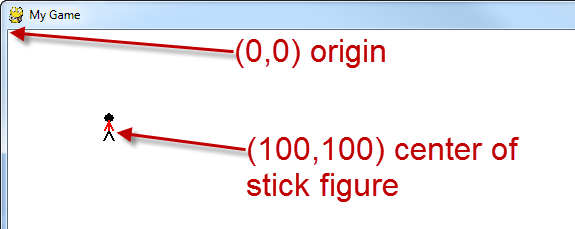
\includegraphics[scale=0.5]{images/positionnement.png}
\end{center}
\end{minipage}

En \texttt{Python}, une matrice de pixels peut être représentée comme un tableau de tableaux, ou liste de listes dans la nomenclature \texttt{Python}. On utilise l'opérateur crochet une fois pour accéder à une ligne par son index et deux fois pour accéder à un pixel par ses index de ligne puis de colonne.


\begin{lstlisting}[style=rond]
>>> pix = [[1, 0, 1, 0], [0, 1, 0, 1]]
>>> pix[0]  #première ligne 
[1, 0, 1, 0]
>>> pix[1] #deuxième ligne
[0, 1, 0, 1]
>>> pix[0][2]  #pixel en 1ere ligne et 3eme colonne
1
\end{lstlisting}


Dans la représentation donnée par \href{http://pythontutor.com}{http://pythontutor.com}, on voit bien que \texttt{pix[0]}, de type \texttt{list}, est une référence vers le tableau de pixels représentant la première ligne. 
\begin{center}
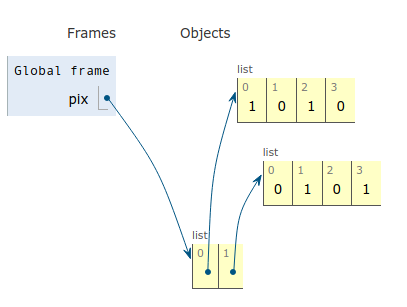
\includegraphics[scale=0.8]{images/exemple_binaire_tutor.png}
\end{center}


\end{cours}

\vspace*{-20pt}

\begin{exercice}{}
\begin{enumerate}
	\item Récupérer l'archive  \texttt{Images-Tableaux2d-materiel.zip}, la copier dans un répertoire pertinent et la déballer.
	\item Ouvrir le fichier \texttt{Images-Tableaux2d-Eleves-Partie1.py} dans un IDE \texttt{Python} et le renommer éventuellement.
	\item 
\begin{enumerate}
\item Créer l'image présentée dans le point de cours 1, en évaluant dans la console l'expression :
\begin{lstlisting}[style=compil]
>>> matrice_to_image([[1,0,1,0],[0,1,0,1]], mode = '1', fichier='exemple_binaire_4x2.png',res=1)
\end{lstlisting}
Un fichier au format \href{https://fr.wikipedia.org/wiki/Portable_Network_Graphics}{PNG} a été créé sur le disque. Il s'agit d'un \textbf{fichier binaire}  lisible uniquement par une machine car il s'agit d'une suite d'\textbf{octets}.
\item Éditer le fichier avec un éditeur hexadécimal comme \href{https://hexed.it/}{https://hexed.it/}.  Voici une capture d'écran du résultat avec $16$ octets par ligne :

\begin{center}
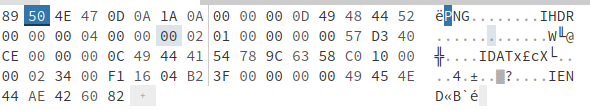
\includegraphics[scale=0.8]{images/exemple_binaire_hex.png}
\end{center}


\item Dans cette question on va décoder le contenu de ce fichier binaire où chaque octet est représenté par un nombre de deux chiffres en hexadécimal.

Ouvrir avec un navigateur web la page d'URL \url{https://fr.wikipedia.org/wiki/Portable_Network_Graphics}

Pourquoi a-t-on créé le format \href{https://fr.wikipedia.org/wiki/Portable_Network_Graphics}{PNG}  ? 

Dans quels cas l'utilise-t-on ?

\item La structure d'un fichier \href{https://fr.wikipedia.org/wiki/Portable_Network_Graphics}{PNG} est la suivante :

\begin{itemize}
	\item signature PNG sur 8 octets
     \item chunk (morceau de fichier) IHDR pour l'en-tête sur  25 octets
     \item chunk IDAT pour les données de longueur variable
     \item chunk IEND pour la fin de fichier sur 12 octets
 \end{itemize}

De plus un chunk est composé de 4 parties :

\begin{center}
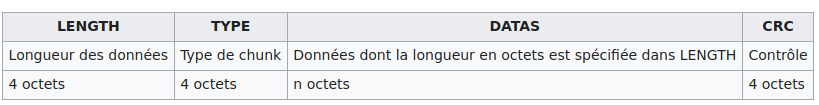
\includegraphics[scale=0.55]{images/chunk-png.png}
\end{center}


Entourer sur la capture d'écran  du fichier, les quatre parties  et les octets représentant respectivement : la largeur, la hauteur, la profondeur de l'image (chunk IHDR), les données (chunk IDAT).

Quel est le rôle des CRC ?


\end{enumerate}
\end{enumerate}



\end{exercice}



\section{Tableaux à 2 ou $n$ dimensions}

\vspace*{-20pt}

\begin{methode}{Manipulations de tableaux à 2 ou $n$ dimensions}

Un tableau \texttt{Python}, de type \texttt{list}, est un conteneur de type séquence qui peut contenir toutes sortes de valeurs, y compris des tableaux. On obtient ainsi une structure de conteneurs imbriqués , on parle de \textbf{tableau à plusieurs dimensions}. Les opérations sur ces tableaux sont les mêmes que sur les tableaux à une dimension présentés dans un chapitre précédent, il faut juste les répéter à chaque niveau d'imbrication. Par exemple \texttt{len} permet d'obtenir la taille d'un tableau qu'il soit conteneur ou élément.

La dimension d'un tableau imbriqué est le nombre de niveaux d'imbrication. Il est possible que tous les éléments n'aient pas la même dimension mais nous ne manipulerons pas ce type de tableaux. 


\begin{itemize}

\item \underline{\textbf{Construction}}

\begin{itemize}

 \item On peut construire un tableau à plusieurs dimensions par \textbf{extension}. Lorsque le tableau a deux dimensions et que toutes les lignes sont de même taille, on peut le qualifier de \textbf{matrice}. 
 
\begin{lstlisting}[style=compil]
>>> t1 = [[1,2], [3,4]]     #tableau/matrice à 2 dimensions
>>> t2 = [[1,2], [3,4],[5,6,7]] #tableau à 2 dimensions
>>> t3 = [[[1], [2,3]],[4,5,6],[7]]  #tableau mixte 
>>> len(t2)    #t2 contient 3 tableaux éléments
3
>>> len(t2[0]) #t2[0] est un tableau contenant 2 entiers
2
>>> len(t2[2]) #t2[2] est un tableau contenant 3 entiers
3

\end{lstlisting}

\item On peut construire un tableau à plusieurs dimensions par \textbf{compréhension} :

\begin{lstlisting}[style=compil]
>>> t4 = [[0] * 3 for _ in range(2)]
>>> t4
[[0, 0, 0], [0, 0, 0]]
>>> t5 = [[ [0] * 4 for i in range(3)] for j in range(2)]
>>> t5
[[[0, 0, 0, 0], [0, 0, 0, 0], [0, 0, 0, 0]], [[0, 0, 0, 0], [0, 0, 0, 0], [0, 0, 0, 0]]]
\end{lstlisting}


\end{itemize}

\item \underline{\textbf{Lecture / écriture}}

On peut lire ou écrire dans un tableau à plusieurs dimensions en traversant les différents niveaux d'imbrication de l'extérieur vers l'intérieur avec l'opérateur crochet :

\begin{lstlisting}[style=compil]
>>> t1[0][1]
2
>>> t1[0][1] = 734
>>> t1
[[1, 734], [3, 4]]
>>> t5[1][2][3] = t1[0][1]
>>> t5
[[[0, 0, 0, 0], [0, 0, 0, 0], [0, 0, 0, 0]], [[0, 0, 0, 0], [0, 0, 0, 0], [0, 0, 0, 734]]]
\end{lstlisting}

\item \underline{\textbf{Parcours}}

Pour parcourir un tableau à plusieurs dimensions, il faut parcourir chaque niveau d'imbrication : par index ou élément par élément. Il faut donc connaître la structure du tableau avant de le parcourir.  

\begin{lstlisting}[style=compil]
>>> def parcours_tableau2d_index(tab):
...     for i in range(len(tab)):
...     	for j in range(len(tab[i])):
...         	print('Element en ligne {} colonne {} : '.format(i,j),tab[i][j])
... 
>>> parcours_tableau2d_index(t1)
Element en ligne 0 colonne 0 :  1
Element en ligne 0 colonne 1 :  734
Element en ligne 1 colonne 0 :  3
Element en ligne 1 colonne 1 :  4
>>> def parcours_tableau2d_element(tab):
...     for ligne in tab:
...             for element in ligne:
...                     print(element)
... 
>>> parcours_tableau2d_element(t1)
1
734
3
4
\end{lstlisting}

\end{itemize}


\end{methode}


\vspace*{-20pt}

\begin{exercice}{}

\begin{enumerate}
	\item Le site \url{http://pythontutor.com/visualize.html} fournit un outil de visualisation de l'état courant d'un programme très pratique. 

Exécutez le code ci-dessous dans \url{http://pythontutor.com/visualize.html#mode=edit} puis commentez.

\begin{lstlisting}[style=rond]
M = [ [0, 0, 0] for i in range(3) ]
N = M
P = [e for e in M ]
Q = [ e[:] for e in M ]
M[2][1] = 3
\end{lstlisting}


\item Compléter la  fonction \texttt{maxi\_tab2d(tab)} pour qu'elle retourne le maximum d'un tableau de nombres à deux dimensions.


\begin{lstlisting}[style=rond]
def max_tab2d(tab):
    """Retourne le maximum d'un tableau à 2 dimensions"""
    maxi = float('-inf')
    for y in range(len(tab)): #boucle sur les lignes
        for x in range(len(tab[y])): # boucle sur les colonnes
            "à compléter"
\end{lstlisting}


Les assertions suivantes doivent être vérifiées :

\begin{lstlisting}[style=rond]
assert max_tab2d([[-1,-2],[-2,-3,-0.5]]) == -0.5
assert max_tab2d([[1,2],[float('inf'),10]]) == float('inf')
assert max_tab2d([[1,2],[8,0]]) == 8
assert max_tab2d([[8, float('-inf')],[]]) == 8
\end{lstlisting}


\item Écrire une fonction  \texttt{moyenne\_tab2d(tab)} qui retourne la valeur moyenne des valeurs  d'un tableau de nombres à deux dimensions.

Les assertions suivantes doivent être vérifiées :

\begin{lstlisting}[style=rond]
assert moyenne_tab2d([[-1,-2],[-2,-3,-0.5]]) == -1.7
assert moyenne_tab2d([[1,2],[float('inf'),10]]) == float('inf')
assert moyenne_tab2d([[1,2],[8,0]]) == 2.75
assert moyenne_tab2d([[8, float('-inf')],[]]) == float('-inf')
\end{lstlisting}


\end{enumerate}


\end{exercice}

\vspace*{-20pt}

\begin{methode}{Copie d'un tableau à plusieurs dimensions}

La valeur d'un tableau étant une référence vers une séquence de données en mémoire, un tableau à deux dimensions est une référence vers une séquence de références, ce qui nécessite un soin particulier pour déréférencer les tableaux imbriqués lors d'une  opération de copie. 

La fonction \texttt{copie\_tab} ci-dessous ne retourne qu'une \textbf{copie superficielle} du tableau passé en paramètre, elle ne déréference pas les éléments du tableau \texttt{M}.


\begin{lstlisting}[style=compil, numbers=left] 
def copie_tab(t):
    res = []
    for x in t:
        res.append(x)
    return res

M = [[1,2],[3,4]]
N = copie_tab(M)
M[0][0] = 0
\end{lstlisting}

\begin{minipage}[t]{0.45\linewidth}
Après l'exécution de la ligne 8, les éléments du tableau \texttt{N}, copie superficielle de \texttt{M}, sont des alias des éléments de \texttt{M} :
\begin{center}
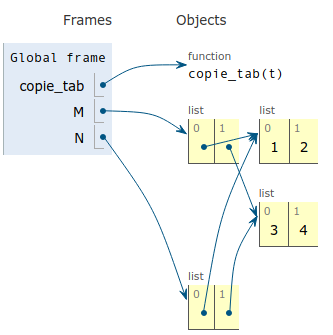
\includegraphics[scale=0.6]{images/copie_tab1.png}
\end{center}
\end{minipage}
\hfill
\begin{minipage}[t]{0.45\linewidth}
Après l'exécution de la ligne 9, la modification de \texttt{M} se traduit par un effet de bord sur \texttt{N} :
\begin{center}
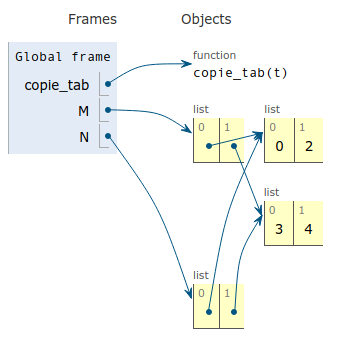
\includegraphics[scale=0.6]{images/copie_tab2.png}
\end{center}
\end{minipage}






\medskip

Pour copier en profondeur un tableau à plusieurs dimensions on peut utiliser la fonction \lstinline{deepcopy} du module \lstinline{copy}.


\medskip

\begin{minipage}{0.95\linewidth}
\begin{lstlisting}[style=compil]  
>>> M = [[1,2],[3,4]]
>>> from copy import deepcopy
>>> N = deepcopy(M)
>>> M[0][0] = 0
>>> N
[[1, 2], [3, 4]]
\end{lstlisting}
\end{minipage}


Une explication très claire du caractère modifiable des listes est donnée dans cette video :

\begin{center}
	\url{https://d381hmu4snvm3e.cloudfront.net/videos/MhgBaG50LRrH/SD.mp4}
\end{center}

\end{methode}


\vspace*{-20pt}



\begin{exercice}{QCM type E3C2}

\begin{enumerate}
\item On considère le tableau \texttt{t} suivant.

\lstinline!t = [[1, 2, 3], [2, 3, 4], [3, 4, 5], [4, 5, 6]]!

Quelle est la valeur de \texttt{t[1][2]} ?

Réponses :

\begin{multicols}{4}

\begin{enumerate}
\item
  1
\item
  3
\item
  4
\item
  2
\end{enumerate}
\end{multicols}

\item Quelle est la valeur de la variable image après exécution du script
Python suivant ?

\begin{lstlisting}[style=rond]
image = [[0, 0, 0, 0], [0, 0, 0, 0], [0, 0, 0, 0], [0, 0, 0, 0]]
for i in range(4):
    for j in range(4):
        if (i+j) == 3:
            image[i][j] = 1
\end{lstlisting}

Réponses :

\begin{enumerate}
\item
  \lstinline![[0, 0, 0, 0], [0, 0, 0, 0], [0, 0, 0, 0], [1, 1, 1, 1]]!
\item
  \lstinline![[0, 0, 0, 1], [0, 0, 0, 1], [0, 0, 0, 1], [0, 0, 0, 1]]!
\item
  \lstinline![[0, 0, 0, 1], [0, 0, 1, 0], [0, 1, 0, 0], [1, 0, 0, 0]]!
\item
 \lstinline![[0, 0, 0, 1], [0, 0, 1, 1], [0, 1, 1, 1], [1, 1, 1, 1]]!
\end{enumerate}


\item On définit une grille G remplie de 0, sous la forme d'une liste de
listes, où toutes les sous-listes ont le même nombre d'éléments.

\begin{lstlisting}[language=Python]
G = [ [0, 0, 0, ..., 0],
[0, 0, 0, ..., 0],
[0, 0, 0, ..., 0],

......
[0, 0, 0, ..., 0]]
\end{lstlisting}

On appelle \emph{hauteur} de la grille le nombre de sous-listes
contenues dans G et \emph{largeur} de la grille le nombre d'éléments
dans chacune de ces sous-listes. Comment peut-on les obtenir ?

Réponses :

\begin{enumerate}
\item
  

\begin{lstlisting}[language=Python]
hauteur = len(G[0])
largeur = len(G)
\end{lstlisting}

\item 

\begin{lstlisting}[language=Python]
hauteur = len(G)
largeur = len(G[0])
\end{lstlisting}

\item 

\begin{lstlisting}[language=Python]
hauteur = len(G[0])
largeur = len(G[1])
\end{lstlisting}

\item 

\begin{lstlisting}[language=Python]
hauteur = len(G[1])
largeur = len(G[0])
\end{lstlisting}
\end{enumerate}


\item 
Quelle est la valeur de l'expression
\lstinline![[0] * 3 for i in range(2)]! ?

Réponses :

\begin{multicols}{2}
\begin{enumerate}

\item
 \lstinline![[0,0], [0,0], [0,0]]!
\item
 \lstinline![[0,0,0], [0,0,0]]!
\item
\lstinline![[0.000], [0.000]]!
\item
 \lstinline![[0.00], [0.00], [0.00]]!
\end{enumerate}
\end{multicols}


\item On exécute le script suivant~:

\begin{lstlisting}[style=rond]
asso = []
L=[['marc','marie'],['marie','jean'],
    ['paul','marie'], ['marie','marie'],
    ['marc','anne']]
for c in L :
    if c[1]=='marie':
        asso.append(c[0])
\end{lstlisting}

Que vaut \texttt{asso} à la fin de l'exécution ?

Réponses :

\begin{enumerate}
\item   \lstinline!['marc', 'jean', 'paul']!
\item \lstinline![['marc','marie'], ['paul','marie'], ['marie','marie']]!
\item \lstinline!['marc', 'paul', 'marie']!
\item \lstinline!['marie', 'anne']!
\end{enumerate}

\end{enumerate}
\end{exercice}

\vspace*{-20pt}

\section{Traitement d'image}

\vspace*{-20pt}


\begin{exercice}{}

Ouvrir le fichier \texttt{Images-Tableaux2d-Eleves-Partie1.py} dans un IDE \texttt{Python}.

\begin{enumerate}
	\item Le prototype d'une fonction doit indiquer son nom, le type de la valeur de retour et le type des paramètres. En \texttt{Python},  la liste des  paramètres suit la déclaration de la fonction avec l'instruction \texttt{def}, les paramètres ne sont pas obligatoirement typés et le type de retour n'est pas précisé mais on doit pouvoir les déduire de la documentation.  
Déterminer le prototype  de la fonction  \texttt{matrice\_to\_image} qui est fournie.
\item Le paramètre \texttt{res} permet de définir le côté en pixels  sur l'écran d'un pixel défini dans la matrice de pixels passée en paramètre. Cela permet de visualiser les images de petites dimensions. L'expression suivante permet d'obtenir l'image du point de cours n°1 avec des blocs de 100 pixels sur l'écran :

\begin{lstlisting}[style=compil]
>> matrice_to_image([[1,0,1,0],[0,1,0,1]], fichier='exemple_binaire.png',res=100)
\end{lstlisting}

Quelle expression permet de générer l'image ci-dessous avec des blocs de 60 pixels écran ?

\begin{center}
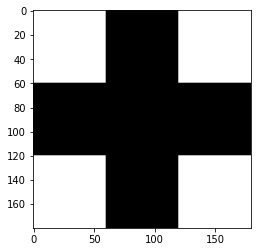
\includegraphics[scale=0.4]{images/croix_binaire.png}
\end{center}
\end{enumerate}


\end{exercice}

\vspace*{-20pt}

\begin{cours}{}
La \textbf{représentation bitmap}   d'une image par une matrice de pixels ne se limite pas à des \textbf{images binaires} en noir (0)  et blanc (1). 

En modifiant la \textbf{profondeur} de l'image, on peut coder plus de couleurs dans un pixel :

\begin{itemize}[label=\ding{43}]
	\item Avec une profondeur de $8$ bits (1 octet), on peut stocker $2^{8}=256$ nuances par pixel. On utilise en général ce mode pour les \textbf{images en nuances de gris}  du plus foncé $0$ (noir) au plus clair $255$ (blanc) mais on le retrouve  pour des images  qui n'ont pas besoin d'une palette de couleurs  étendue  comme dans le format \href{https://fr.wikipedia.org/wiki/Graphics_Interchange_Format}{GIF}.
	
\begin{minipage}{0.65\linewidth}
Expression pour générer l'image en niveaux de gris ci-contre :

\begin{lstlisting}[style=compil]
>>> pix = [[0,50,100],[150,200,255]]
>>> matrice_to_image(pix,mode = 'L', 
fichier='exemple.png',res=100)
\end{lstlisting}
\end{minipage}
\hfill
\begin{minipage}{0.3\linewidth}
\begin{center}

\includegraphics[scale=0.5]{images/exemple_grayscale.png}
\end{center}
\end{minipage}

	\item Avec une profondeur de $24$ bits (3 octets), on peut stocker $2^{24} \approx 16 \times 10^{6}$ nuances par pixel. En général on utilise ce mode pour la représentation des couleurs par \href{https://fr.wikipedia.org/wiki/Synth\%C3\%A8se_additive}{synthèse additive} de trois couleurs primaires (Rouge, Vert, Bleu). Un pixel est alors représenté par une liste de trois entiers entre $0$ et $255$ pour mesurer les intensités des trois composantes.
	
\begin{minipage}{0.65\linewidth}
Expression pour générer l'image en couleurs ci-contre :

\begin{lstlisting}[style=compil]
>>> pix = [
			[[255,0,0],[0,255,0]],
			[[0,0,255],[255,255,255]]
		  ]
>>> matrice_to_image(pix,mode = 'RGB', 
fichier='exempleRGB.png',res=100)
\end{lstlisting}
\end{minipage}
\hfill
\begin{minipage}{0.3\linewidth}
\begin{center}

\includegraphics[scale=0.5]{images/exempleRGB.png}
\end{center}
\end{minipage}

\end{itemize}


\end{cours}

\vspace*{-20pt}


\begin{exercice}{}

Compléter le code de la procédure \texttt{generer\_croix} pour qu'elle génère une image de croix avec la couleur passée en paramètre :

\begin{lstlisting}[style=rond]
def generer_croix(couleur):
    blanc = [255,255,255]
    croix = ..............
    matrice_to_image(croix, mode = 'RGB', res = 10, fichier='croix.png')  
\end{lstlisting}

Par exemple, l'évaluation de \texttt{croix([255,0,0])} donne :
\begin{center}

\includegraphics[scale=0.2]{images/croix.png}
\end{center}

\end{exercice}

\vspace*{-20pt}


\begin{exercice}{}




\begin{enumerate}
 \item Compléter le code de la fonction \texttt{matrice\_vide} pour qu'elle retourne une matrice de pixels représentant une image noire dans le mode choisi (\texttt{'1'}, \texttt{'L'} ou \texttt{'RGB'}) avec \texttt{nlig} lignes et \texttt{ncol} colonnes :

\begin{lstlisting}[style=rond]
def matrice_vide(ncol, nlig, mode):
    """Retourne une matrice de pixels de n lignes et m colonnes
    représentant une image noire dans le mode  d'image choisi"""
    assert mode in ['1', 'L', 'RGB'], "mode doit appartenir à ['1', 'L', 'RGB']"
    #compléter par des tableaux définis en compréhension
    if mode in ['1', 'L']:
        return .........................
    else:               
        return ..........................
\end{lstlisting}

	\item Compléter le code de la fonction \texttt{drapeau\_3bandes\_verticales} ci-dessous pour que cette expression génère le drapeau national :

\begin{lstlisting}[style=compil]
matrice_to_image(drapeau_3bandes_verticales(3,6,[0,0,255],[255,255,255], [255,0,0]), mode='RGB', fichier='drapeau-france.png', res = 100)
\end{lstlisting}


\begin{lstlisting}[style=rond]
def drapeau_3bandes_verticales(nlig, ncol, couleur1, couleur2, couleur3):
    #on crée une matrice vide de bonnes dimensions
    pix = matrice_vide(ncol, nlig, 'RGB')
    tiers_colonne = ncol // 3
    deux_tiers_colonne = 2 * tiers_colonne
    for x in range(ncol): #boucle sur les colonnes
        for y in range(nlig): #boucle sur les lignes
            if   x < tiers_colonne:
                pix[y][x] = couleur1
            #à compléter !
    return pix
\end{lstlisting}

   \item Écrire une fonction \texttt{transpose(pix, mode)} qui échange les lignes et les colonnes de la matrice de pixels passée en paramètre. La matrice de pixels \texttt{tpix} retournée est  telle que la valeur \texttt{tpix[y][x]} est celle de \texttt{pix[x][y]}.


On utilisera la fonction \texttt{matrice\_vide} et la fonction \texttt{dimensions} qui est fournie :

\begin{lstlisting}[style=rond]
def dimensions(pix):
    "Retourne les dimensions (Largeur, Hauteur) de la matrice pix"
    return len(pix[0]), len(pix) 
\end{lstlisting}

La série d'assertions ci-dessous doit être vérifiée par la fonction \texttt{transpose} :

\begin{lstlisting}[style=compil]
assert transpose([[0]],'L') == [[0]]
assert transpose([[1,2],[4,5]], 'L') == [[1,4],[2,5]]
assert transpose([[1,2,3],[4,5,6]],'L') == [[1,4],[2,5],[3,6]]
assert transpose([[[1,2,3],[4,5,6]],[[7,8,9],[10,11,12]]],'RGB') == [[[1,2,3],[7,8,9]],[[4,5,6],[10,11,12]]]
\end{lstlisting}
 
   \item En déduire l'écriture d'une fonction \texttt{drapeau\_3bandes\_horizontales}, telle que cette expression génère le drapeau de la Hollande :
   
\begin{lstlisting}[style=compil]
matrice_to_image(drapeau_3bandes_horizontales(3,6,[255,0,0], [255,255,255],[0,0,255]),mode='RGB', fichier='drapeau-hollande.png', res = 100)
\end{lstlisting}

\end{enumerate}
\end{exercice}


\vspace*{-20pt}


\begin{exercice}{}

L'opérateur  modulo \% permet de calculer le reste de la division euclidienne d'un entier \texttt{a} par un entier \texttt{b} avec la syntaxe \texttt{a \% b}. On peut ainsi évaluer la parité d'un entier.

\begin{lstlisting}[style=compil]
>>> 7 % 2
1
>>> 8 % 2
0
\end{lstlisting}


Dans cet exercice, on travaille sur des images binaires avec deux couleurs possibles noir (0) ou blanc (1).

\begin{enumerate}
	\item Compléter la fonction \texttt{barres\_horizontales} pour qu'elle retourne la matrice de pixels d'une image  de dimensions  \texttt{ncol} $\times$ \texttt{nlig}  avec alternance   de lignes noires (index pair)  ou blanches (index impair).

\begin{lstlisting}[style=rond]
def barres_horizontales(nlig, ncol):
    #on crée une matrice vide de bonnes dimensions
    pix = matrice_vide(ncol, nlig, '1')
    for x in range(ncol): #boucle sur les colonnes
        for y in range(nlig): #boucle sur les lignes
            "à compléter"
    return pix 
\end{lstlisting}

L'expression \lstinline+matrice_to_image(barres_horizontales(4, 5), mode='1', res = 50)+ génère cette image (sans le cadre orange) :
\begin{center}

\includegraphics[scale=0.5]{images/bandes-horizontales-cadre.png}
\end{center}
\item Écrire une fonction \texttt{damier(nlig, ncol)} qui retourne la matrice de pixels permettant de générer un damier de cases blanches et noires avec \texttt{nlig} lignes et \texttt{ncol} colonnes.

L'expression \lstinline+matrice_to_image(damier(4,8), mode='1', res = 50)+ doit générer l'image ci-dessous (sans le cadre orange) :

\begin{center}

\includegraphics[scale=0.5]{images/damier-cadre.png}
\end{center}
\end{enumerate}

\end{exercice}

\vspace*{-20pt}

\begin{exercice}{Filtre pixel par pixel}

La fonction \texttt{applique\_filtre} permet d'appliquer une fonction (ou filtre) à chaque pixel d'une matrice de pixels et de retourner une nouvelle matrice de mêmes dimensions avec les pixels transformés. Le paramètre \texttt{mode} désigne le mode de l'image transformée qui peut être différent de celui de l'image source.

\begin{lstlisting}[style=rond]
def applique_filtre(pix, filtre, mode):
    ncol, nlig = dimensions(pix)
    pix_but = matrice_vide(ncol, nlig, mode)
    for x in range(ncol): #boucle sur les colonnes
        for y in range(nlig): #boucle sur les lignes
            pix_but[y][x] = filtre(pix[y][x])
    return pix_but

def filtre_negatif_gris(pixel):
    """Filtre négatif pour image en niveaux de gris"""
    return 255 - pixel
\end{lstlisting} 


\begin{enumerate}
	\item Avec la fonction \texttt{filtre\_negatif\_gris}, on peut générer le négatif d'une image en niveaux de gris comme \texttt{exemple\_gris.png} qui est fournie. Exécuter la séquence d'instructions ci-dessous :

\begin{lstlisting}[style=compil]
>>> exemple_gris = image_to_matrice('exemple_gris.png')
>>> exemple_gris_negatif = applique_filtre(exemple_gris, filtre_negatif_gris, 'L')
>>> matrice_to_image(exemple_gris_negatif, fichier='exemple_gris_negatif.png', mode='L', res=1)
\end{lstlisting}

\begin{minipage}{0.45\linewidth}

\begin{center}
exemple\_negatif.png

\medskip


\includegraphics[scale=0.5]{images/exemple_gris.png}
\end{center}
\end{minipage}\hfill
\begin{minipage}{0.45\linewidth}
\begin{center}
exemple\_gris\_negatif.png

\medskip


\includegraphics[scale=0.5]{images/exemple_gris_negatif.png}
\end{center}
\end{minipage}

\item Écrire une fonction \texttt{filtre\_negatif\_rgb} qui associe à la valeur d'un pixel en RGB son négatif.

L'assertion ci-dessous doit être vérifiée :

\begin{lstlisting}[style=compil]
assert filtre_negatif_rgb([255,0,100]) == [0,255,155]
\end{lstlisting}

Tester cette fonction  sur l'image fournie \texttt{cardinal.jpg} représentant le  \og{} Cardinal Fernando Niño de Guevara (1541–1609) \fg{} peint par  \textit{El Greco } {\footnotesize Metropolitan Museum of New York licence CC0 1.0} %\footnote{Metropolitan Museum of New York licence CC0 1.0}.

\begin{lstlisting}[style=compil]
>>> cardinal = image_to_matrice('cardinal.jpg')
>>> cardinal_negatif = applique_filtre(cardinal, filtre_negatif_rgb, 'RGB')
>>> matrice_to_image(cardinal_negatif, fichier='cardinal-negatif.png', mode='RGB',res=1)
\end{lstlisting}


\begin{minipage}{0.45\linewidth}
\begin{center}
\textbf{Original}

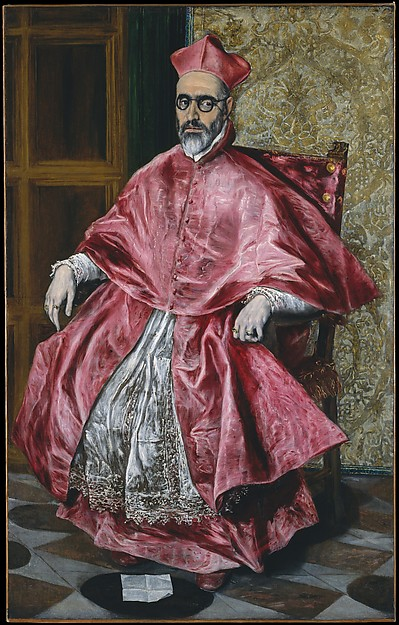
\includegraphics[scale=0.5]{images/cardinal.jpg}
\end{center}
\end{minipage}\hfill
\begin{minipage}{0.45\linewidth}
\begin{center}
\textbf{Négatif}

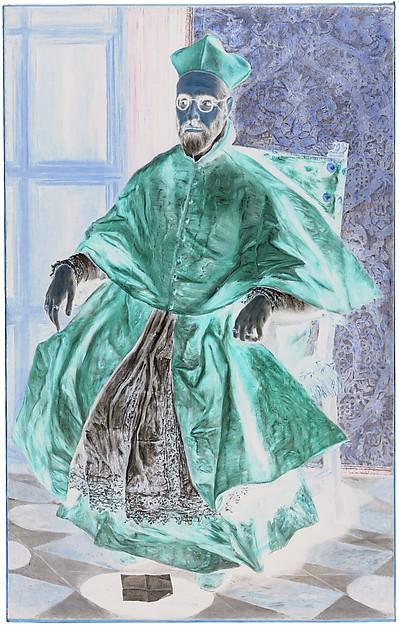
\includegraphics[scale=0.25]{images/cardinal-negatif.png}
\end{center}
\end{minipage}

\item Écrire une fonction \texttt{fonction\_seuil(val, seuil, vmin, vmax)} qui retourne \texttt{vmin} si \texttt{val <= seuil} et \texttt{vmax} sinon.

On donne la  fonction \texttt{filtre\_seuillage\_gris} qui retourne une fonction de filtre permettant d'associer à un pixel en nuance de gris soit 0 (noir) s'il est foncé par rapport au seuil,  soit 255 (blanc) s'il est clair. 

Cette méthode permet de fixer un paramètre dans une fonction à deux paramètres.

\begin{lstlisting}[style=rond]
def filtre_seuillage_gris(seuil):
    def f(pixel):
        return fonction_seuil(pixel, seuil, 0, 255)    
    return f
\end{lstlisting}

L'image en nuances de gris \texttt{lena.png} est fournie. Exécuter la séquence d'instructions ci-dessous, on peut séparer, selon un seuil, les pixels d'une image en deux catégories  : les clairs et les foncés.

\begin{lstlisting}[style=compil]
>>> lena = image_to_matrice('lena.png')
>>> lena_seuil = applique_filtre(lena, filtre_seuillage_gris(100), 'L')
>>> matrice_to_image(lena_seuil, fichier = 'lena-seuil.png', mode = 'L', res = 1)
\end{lstlisting}



\begin{minipage}{0.45\linewidth}
\begin{center}
\textbf{Original}

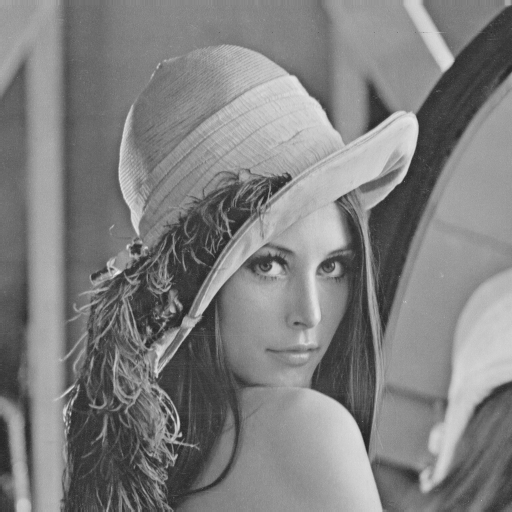
\includegraphics[scale=0.25]{images/lena.png}
\end{center}
\end{minipage}\hfill
\begin{minipage}{0.45\linewidth}
\begin{center}
\textbf{Avec un seuillage de 100}

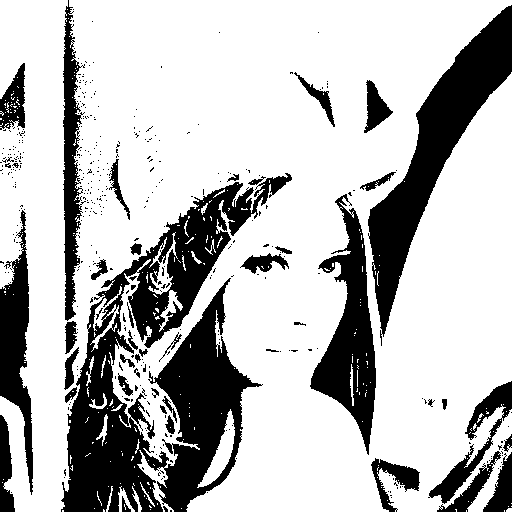
\includegraphics[scale=0.25]{images/lena-seuil.png}
\end{center}
\end{minipage}


\item

\begin{enumerate}
\item  Écrire une fonction \texttt{filtre\_rouge} qui prend en paramètre un pixel RGB, sous forme de liste \texttt{[r,g,b]} de trois entiers entre 0 et 255, et retourne sa projection sur la composante rouge \texttt{[r,0,0]}.


Les assertions suivantes doivent être  vérifiées.

\begin{lstlisting}[style=rond]
assert filtre_rouge([255,0,0]) == [255,0,0]
assert filtre_rouge([255,255,0]) == [255,0,0]
assert filtre_rouge([255,255,255]) == [255,0,0]
assert filtre_rouge([0,255,0]) == [0,0,0]
\end{lstlisting}

Exécuter la séquence d'instructions ci-dessous, on peut ainsi extraire l'image constituée de toutes les  composantes rouges des pixels d'une image RGB 

\begin{lstlisting}[style=compil]
>>> cardinal_rouge = applique_filtre(cardinal, filtre_rouge, 'RGB')
>>> matrice_to_image(cardinal_rouge, mode ='RGB', res= 1, fichier='cardinal-rouge.png')
\end{lstlisting}


\begin{minipage}{0.45\linewidth}
\begin{center}
\textbf{Original}

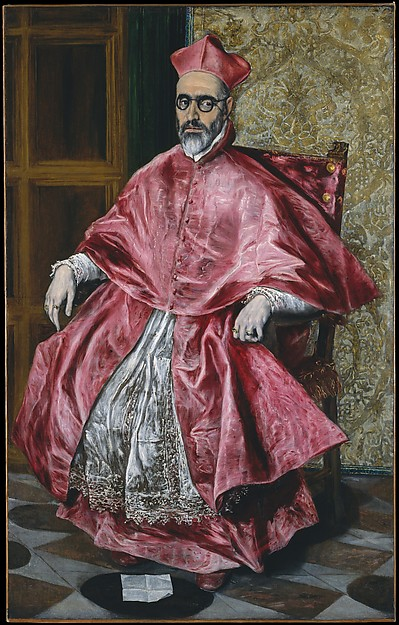
\includegraphics[scale=0.5]{images/cardinal.jpg}
\end{center}
\end{minipage}\hfill
\begin{minipage}{0.45\linewidth}
\begin{center}
\textbf{Composante rouge} 

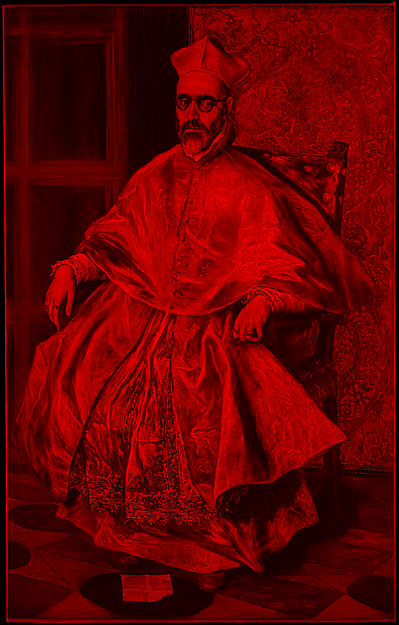
\includegraphics[scale=0.25]{images/cardinal-rouge.png}
\end{center}
\end{minipage}

\item Sur le modèle de la fonction \texttt{filtre\_seuillage\_gris}, écrire une fonction \texttt{filtre\_composante\_rgb(index\_comp)} qui retourne la  fonction de filtre de composante pour un pixel en RGB correspondant à l'index de la composante passé en paramètre.

La fonction doit vérifier les assertions suivantes :

\begin{lstlisting}[style=rond]
assert filtre_composante_rgb(0)([255,200,100]) == [255,0,0]
assert filtre_composante_rgb(1)([255,200,100]) == [0,200,0]
assert filtre_composante_rgb(2)([255,200,100]) == [0,0,100]
\end{lstlisting}

Extraire les composantes bleue et verte de l'image \texttt{cardinal.jpg} et les enregistrer sur le disque.

\end{enumerate}

\item 

\begin{enumerate}
	\item Compléter la fonction  de filtre de pixel \texttt{filtre\_monochrome} qui retourne la moyenne pondérée des composantes d'un pixel RGB par les coefficients \texttt{[0.299,0.587,0.114]} qui sont habituellement utilisés pour convertir une image RGB en nuances de gris.
	
\begin{lstlisting}[style=rond]
def filtre_monochrome(pixel_rgb):
    """Retourne la moyenne pondérée des composantes
    d'un pixel RGB par les coefs [0.299,0.587,0.114]"""
    coef = [0.299,0.587,0.114]
    pixel_gris = 0
    somme_coef = 0
    "à compléter"
\end{lstlisting}

Les assertions suivantes doivent être vérifiées :

\begin{lstlisting}[style=rond]
assert filtre_monochrome([255,100,200]) == 157
assert filtre_monochrome([200,255,100]) == 220
assert filtre_monochrome([100,200,255]) == 176
\end{lstlisting}

\item Utiliser la fonction \texttt{filtre\_monochrome} pour générer et enregistrer sur le disque la conversion en nuances de gris de l'image \texttt{cypres.jpg} représentant un  tableau peint par Vincent Van Gogh,  {\footnotesize Metropolitan Museum of New York licence CC0 1.0}.

\begin{minipage}{0.45\linewidth}
\begin{center}
\textbf{Original en couleur}
 
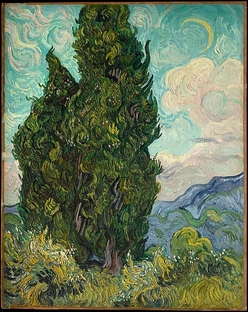
\includegraphics[scale=1]{images/cypres-tiny.jpg}
\end{center}
\end{minipage}\hfill
\begin{minipage}{0.45\linewidth}
\begin{center}
\textbf{Nuances  de gris}

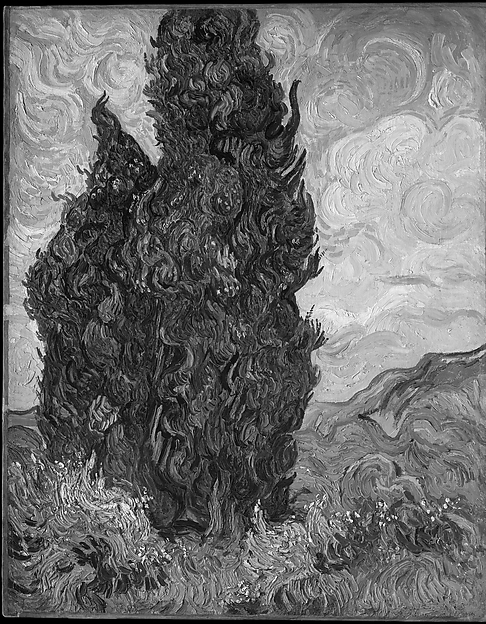
\includegraphics[scale=0.25]{images/cypres-gris.png}
\end{center}
\end{minipage}


\end{enumerate} 

\end{enumerate}



\end{exercice}



\newpage

\tableofcontents
 \end{document}
